\documentclass[a4paper,11pt,pdftex,accentcolor=tud2d,article,parskip,colorbacktitle, type=msc]{tudthesis}
\usepackage[ngerman,english]{babel}
%\documentclass[article,dr=phil,type=drfinal,colorback,accentcolor=tud9c]{tudthesis}
%\usepackage{ngerman}
\newcommand{\getmydate}{%
  \ifcase\month%
    \or Januar\or Februar\or M\"arz%
    \or April\or Mai\or Juni\or Juli%
    \or August\or September\or Oktober%
    \or November\or Dezember%
  \fi\ \number\year%
}

%%%%%%%%%%%%%%%%%%%%%%%%%%%%%%%%%%%%%%%%%%%%%%%%%%%%%%%%%
%%%%%%%%%%% FILL THIS OUT %%%%%%%%%%%%%%%%%%%%%%%%%%%%%%%
%%%%%%%%%%%%%%%%%%%%%%%%%%%%%%%%%%%%%%%%%%%%%%%%%%%%%%%%%
% thesis language
\selectlanguage{english}
% title in english
\def\TitleEnglish{Secure IoT Applications Using Scalable Blockchain Models And PQ Primitives}
% title in german (leave this blank if you dont want one)
\def\TitleGerman{Sichere IoT Anwendungen unter Nutzung skalierbarer Blockchain Modelle und PQ Primitive}
% short author name
\def\AuthorShort{Muhammad Rameez}
% full author name
\def\AuthorLong{Muhammad Rameez}
% the hand in date
\def\HandInDate{24th September 2018}
% first referee
\def\GutachterOne{Prof. Johannes Buchmann}
% second referee
\def\GutachterTwo{Dr. Rachid El Bansarkhani}
% advisor
\def\Betreuer{Dr. Rachid El Bansarkhani}
%%%%%%%%%%%%%%%%%%%%%%%%%%%%%%%%%%%%%%%%%%%%%%%%%%%%%%%%%
%%%%%%%%%%%%%%%%%%%%%%%%%%%%%%%%%%%%%%%%%%%%%%%%%%%%%%%%%
%%%%%%%%%%%%%%%%%%%%%%%%%%%%%%%%%%%%%%%%%%%%%%%%%%%%%%%%%

% Header file defines all packages, defines variables, ...
\definecolor{secusoblue}{RGB}{0,67,101}
\makeatletter\renewcommand{\TUD@accentcolor}{\color{secusoblue}}\renewcommand{\TUD@identbarcolor}{\color{secusoblue}}\makeatother
\usepackage[utf8]{inputenc}
\usepackage[T1]{fontenc}
\usepackage[english=american]{csquotes}
%\usepackage[sort]{natbib}
% Paket setspace erlaubt Umschalten auf 1.5fachen Zeilenabstand
\usepackage{setspace}
\onehalfspacing %Zeilenabstand wird global auf 1.5 festgelegt

% Great package for creating pictures, graphs, etc. (check the web for examples!)
  \usepackage{tikz}
\usetikzlibrary{intersections,calc}

% Some general packages for tables, formulas, creation of booktabs etc.
\usepackage{tabularx}
\usepackage{longtable}
\usepackage{multirow}
\usepackage{booktabs}
\usepackage{amsmath}
\usepackage{amsxtra}
\usepackage{enumitem}

%custom packages added by rameez
%\usepackage{cite}
\usepackage{acronym}
\usepackage{listings}
\usepackage{url}
%\usepackage{hyperref}
\usepackage{graphicx}
\usepackage{placeins}
\usepackage{float}
\usepackage{makeidx}
\usepackage{lipsum}
\usepackage{amsmath}
\usepackage{filecontents}

\raggedbottom
\parindent 0pt

% Package to include tables (e.g. figures) in the table of contents
\usepackage[nottoc]{tocbibind} 

% Institution logo (if not defined, uses department and group text)
\setinstitutionlogo{figs/tud_logo}

\thesistitle{\TitleEnglish}{\TitleGerman}
\author{\AuthorShort\\ Matriculation No.: 2556345}
\referee{\GutachterOne}{\GutachterTwo\\ Betreuer: \Betreuer}
\department{Fachbereich Informatik}
\group{CDC – Theoretische Informatik – Kryptographie und Computeralgebra}

\newcommand{\stafford}[1]{\fontfamily{5sf} \selectfont #1 \fontfamily{5ch}\selectfont}

\usepackage[colorlinks=true,
                pdftex,
                pdfstartview=FitB,
                pdffitwindow=true,
                bookmarksopen=true,
                linkcolor=black,
                citecolor=black,
                breaklinks=true,
                % Title
                pdftitle={\TitleEnglish},
                % Author
                pdfauthor={\AuthorLong, Technische Universit\"at Darmstadt}]{hyperref}

\usepackage{hyperref}
\usepackage[a-1b]{pdfx}
\begin{document}
%%%%%%%%%%%%%%%%%%%%%%%%%%%%%%%%%%%%%%%%%%%%%%%%%%%%%%%%%
%%%%%%%%%%% for hyphentations %%%%%%%%%%%%%%%%%%%%%%%%%%%
%%%%%%%%%%%%%%%%%%%%%%%%%%%%%%%%%%%%%%%%%%%%%%%%%%%%%%%%%
  % If you want to define hyphenations (optional)
  % \hyphenation{
  % Some examples for hyphenations
  In-for-ma-tions-sicher-heits-ma\ss nahmen
  In-for-ma-tions-sicher-heit
  Organisations-rollen
}
%%%%%%%%%%%%%%%%%%%%%%%%%%%%%%%%%%%%%%%%%%%%%%%%%%%%%%%%%
%%%%%%%%%%%%%%%%%%%%%%%%%%%%%%%%%%%%%%%%%%%%%%%%%%%%%%%%%

%%%%%%%%%%%%%%%%%%%%%%%%%%%%%%%%%%%%%%%%%%%%%%%%%%%%%%%%%
%%%%%%%%%% additional logos %%%%%%%%%%%%%%%%%%%%%%%%%%%%%
%%%%%%%%%%%%%%%%%%%%%%%%%%%%%%%%%%%%%%%%%%%%%%%%%%%%%%%%%
  % Input logo(s) -> necessary if you want to insert several logos
  % put needs a definition of the position!
  % \sponsor{  
  %     \begin{picture}(,)
  %             \put(399,255){\includegraphics[height=1.4cm]{gfx/logo2}}
  %     \end{picture}
  % }
%%%%%%%%%%%%%%%%%%%%%%%%%%%%%%%%%%%%%%%%%%%%%%%%%%%%%%%%%
%%%%%%%%%%%%%%%%%%%%%%%%%%%%%%%%%%%%%%%%%%%%%%%%%%%%%%%%%

% make title page
\makethesistitle
\affidavit[\today]{\AuthorLong}

%%%%%%%%%%%%%%%%%%%%%%%%%%%%%%%%%%%%%%%%%%%%%%%%%%%%%%%%%
%%%%%%%%%% Abstract %%%%%%%%%%%%%%%%%%%%%%%%%%%%%%%%%%%%%
%%%%%%%%%%%%%%%%%%%%%%%%%%%%%%%%%%%%%%%%%%%%%%%%%%%%%%%%%
\pagestyle{empty}
%\begin{abstract}
\begin{abstract}
In this paper, I explore different blockchain technologies and how they can be exploited for different use case scenarios. I mainly focus on 4 use cases namely Supply Chain Management, Internet of things, File Sharing and Machine to Machine. First, a general introduction of the blockchain is presented. Then, I discuss Ethereum and Smart contracts and what makes it different compared to Bitcoin. I highlight some of the challenges facing blockchains today i.e. the scaling problem, and the transaction finality issue. Then, I look at possible solutions proposed by Ethereum and Bitcoin in order to tackle these problems. A possible extension to one of these solutions in the form of virtual channels and Perun is explored next. Finally, I explore four use case scenarios of blockchains in industry and how it is helping to transform them in each case. 
\end{abstract}
%\end{abstract}
\newpage
%%%%%%%%%%%%%%%%%%%%%%%%%%%%%%%%%%%%%%%%%%%%%%%%%%%%%%%%%
%%%%%%%%%%%%%%%%%%%%%%%%%%%%%%%%%%%%%%%%%%%%%%%%%%%%%%%%%

%%%%%%%%%%%%%%%%%%%%%%%%%%%%%%%%%%%%%%%%%%%%%%%%%%%%%%%%%
%%%%%%%%%% Preface %%%%%%%%%%%%%%%%%%%%%%%%%%%%%%%%%%%%%
%%%%%%%%%%%%%%%%%%%%%%%%%%%%%%%%%%%%%%%%%%%%%%%%%%%%%%%%%
\pagestyle{empty}
%\begin{Preface}
%\include{chapters/Preface}
%\end{Preface}
\newpage
%%%%%%%%%%%%%%%%%%%%%%%%%%%%%%%%%%%%%%%%%%%%%%%%%%%%%%%%%
%%%%%%%%%%%%%%%%%%%%%%%%%%%%%%%%%%%%%%%%%%%%%%%%%%%%%%%%%
% Crate content table
\tableofcontents
\newpage

  
% Adjust page numbering (optional)
\pagenumbering{arabic}
\pagestyle{plain}
  
%%%%%%%%%%%%%%%%%%%%%%%%%%%%%%%%%%%%%%%%%%%%%%%%%%%%%%%%%
%%%%%%%%%% Content %%%%%%%%%%%%%%%%%%%%%%%%%%%%%%%%%%%%%%
%%%%%%%%%%%%%%%%%%%%%%%%%%%%%%%%%%%%%%%%%%%%%%%%%%%%%%%%%
\section{Introduction And Motivation}
\subsection{Introduction To Blockchain}
\textit{“Blockchain is a continuously growing list of records, called blocks, which are linked and secured using cryptography. Each block contains typically a hash pointer as a link to a previous block, a timestamp and transaction data”} \cite{wiki:001}. It can serve as a distributed ledger that can record transactions without a central server or trusted third party. The transactions are available to all parties and are easily verifiable. It is inherently resistant to data tampering as altering data in any one block breaks the chain and requires that all subsequent blocks be calculated again using the new data. Technical details of blockchains are discussed in chapter \ref{Blockchain}, however for a high level overview please refer to figure \ref{fig:blockchain}. Notice that each block has a unique signature or hash and is linked to previous blocks through its hash. Blockchain has the power to revolutionize how business is conducted in the digital age. Some people are calling it the most important innovation since the development of the internet and the world wide web. The proponents of this technology believe that it will fundamentally transform the web itself. Internet of tomorrow will be powered by decentralized applications or Dapps \cite{misc:020}. The first blockchain was Bitcoin, it was invented by a person or group of persons known only by the pseudonym Satoshi Nakamoto. Bitcoin is a form of peer-to-peer electronic cash designed to transfer value between two parties without involving banks or other financial institutions. It was the first to solve the double spend problem without using a central server. Bitcoin paved the way for exponential growth in crypto currency market which together with other Altcoins is worth over 120 billion dollars at the time of writing. The underlying technology which powers Bitcoin, Ethereum and other crypto currencies can be used for much more than just transferring X amount of coins from Person A to Person B. Researchers are employing blockchain technologies to increase efficiency and reduce costs in industries such as Supply Chain Management, Internet of things, Banking and Finance to name a few.

\begin{figure}[b]
	\centering
    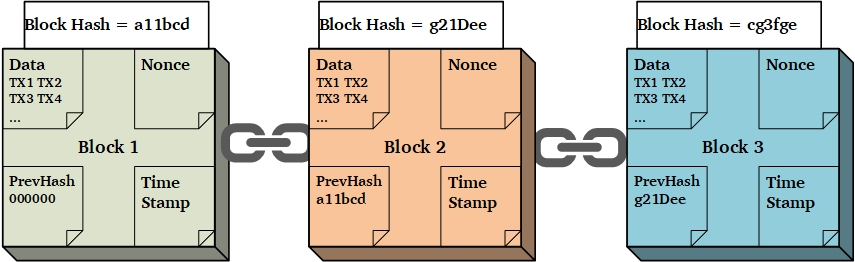
\includegraphics[width=160mm,scale=0.5]{figs/blockchain}
	\caption{High Level Overview of the Blockchain}
	\label{fig:blockchain}
\end{figure}
\clearpage  
\subsection{Blockchain Types}
Blockchain technologies have experienced rapid growth in the recent years. The rapid pace of innovation has given rise to new models, paradigms and technologies in this sector. We now have multiple competing blockchain networks and solutions jostling for different segments of the market. There is Monero and Zcash focusing on privacy oriented solutions employing technologies like ring signatures \cite{paper:008} and zk-SNARKS. Others like Ripple and Hyper Ledger are tailoring their solutions for specific segments of the market like banking and enterprise. This accelerated pace of innovation has ignited a fierce debate in the community as to what can and cannot be classified as a blockchain. The classification schemes consider range of different factors,  including design and architecture of the underlying blockchain protocol. In the paper presented in \cite{7930224} the authors classify blockchain systems based on their architecture and the level of decentralization i.e. Fully Centralized, Partially Decentralized, and Fully Decentralized. Most publications and experts however, classify blockchains into two broad categories: Public or Permissionless Blockchains, and Private or Permissioned Blockchains \cite{misc:017}. This classification is useful as it uses a range of functional and non-functional properties of blockchain systems for categorizing them.
%\bigskip
\vspace{1cm}
\begin{table}[h]
\begin{tabular}{|l|l|l|}
\hline
                          & \multicolumn{1}{c|}{\textbf{Permissionless Blockchains (Public)}} & \multicolumn{1}{c|}{\textbf{Permissioned Blockchains (Private)}} \\ \hline
\textbf{Network Access}   & Any one can join the network                                      & Only authorized participants can join                            \\ \hline
\textbf{Minning}          & Any one can produce new blocks                                    & Authorized block producers                                       \\ \hline
\textbf{Decentralization} & Fully decentralized system                                        & Can have limited to no decentralization                          \\ \hline
\textbf{Speed}            & Slower compared to private blockchains                            & Faster                                                           \\ \hline
\textbf{Transparency}     & Fully transaparent                                                & Customizable level of transparency                               \\ \hline
\end{tabular}
\caption {Permissioned vs Permissionless Blockchains}
\end{table}
%\clearpage  
\vspace{1cm}
\subsubsection{Permissionless Blockchains} 
Permissionless or Public blockchains are highly decentralized networks that value decentralization and censorship resistance above everything else. Permissionless systems allow any person or entity to interact with the network or run smart contracts \cite{arXiv:1806.03693}. Every participant has equal rights to create, send, and view transactions. They can even choose to become block producers or miners and verify transactions in order to append them to the blockchain. 

Bitcoin was the first public blockchain and a realization of a vision outlined by Satoshi in his white paper \cite{paper:001}. He identified decentralization, censorship resistance and distributed trust as the most important factors for the success of the peer-to-peer digital cash protocol he proposed. The main functional and non-functional properties of permissionless systems are given below:
\clearpage
\textbf{Decentralization:}
Public blockchains are usually highly distributed and decentralized. This makes the network censorship resistant and harder to attack and bring down by any one entity. 

\textbf{Consensus Mechanisms:}
Decentralization is achieved at the cost of higher complexity hence public blockchains requires sophisticate consensus mechanisms. There are two main types of consensus mechanisms: Proof of Work [\ref{PW}], and Proof of Stake [\ref{PS}]. Any participating node can run the consensus software in order to verify transactions and extend the blockchain \cite{arXiv:1806.03693}, \cite{misc:017}.

\textbf{Block Producers:}
Any node can choose to become a block producer or miner. Public blockchains usually employ a crypto economic model where by miners are rewarded using network assets or tokens \cite{paper:001}.

\textbf{Privacy:}
Without a central entity or coordinator, transparency becomes an important feature for the participants and miners for establishing trust in the system. This transparency is often achieved by sacrificing some degree of privacy. By default, all transactions and data in a blockchain is public and can be easily accessed with the help of a block explorer.  
\vspace{1cm}
\subsubsection{Permissioned Blockchains}
Permissioned blockchains are sometimes also referred to as private blockchains. It is a closed ecosystem where participants need permission from an administrator or special node to interact with the ledger. Only pre-approved nodes or block producers can verify transactions and run smart contracts \cite{arXiv:1806.03693}. Participants place some level of trust in these block validators or administrators. 

Permissioned blockchains can be managed by members of a consortium in order to increase transparency and efficiency of inter organizational processes. They allow organizations to have better control over proprietary data while facilitating trusted exchange of secure information across organizational hierarchy \cite{arXiv:1806.03693}, \cite{misc:017}. The main functional and non-functional properties of permissioned blockchain systems are given below: 

\textbf{Decentralization:}
Permissioned systems can have varying degrees of decentralization. They can be fully centralized or partially decentralized. Systems like Hyperledger fabric allow fine grained control over governance models and the level of decentralization. The level of decentralization in permissioned systems depends upon many factors including number of participants, their relationship with each other, degree of required fault tolerance, business rules and consensus algorithms \cite{arXiv:1806.03693}, \cite{misc:017}.
\clearpage
\textbf{Consensus Mechanisms:}
Permissioned blockchains usually do not need to run complex consensus algorithms. They can run simplified consensus mechanisms. This coupled with the fact that only a limited number of nodes are responsible for producing new blocks helps them become more efficient and scalable \cite{arXiv:1806.03693}, \cite{misc:017}. 

\textbf{Block Producers:}
Private blockchains can set out criteria for participants to become block producers. These criteria can be based on certain business rules or participating nodes might be required to meet special conditions in order to become block producers such as demonstrating certain capabilities like minimum hash power, or having possession of certain assets etc. Unlike public blockchains block producers are not rewarded with network assets rather they work together to increase efficiency, reduce business costs and boost productivity \cite{arXiv:1806.03693}, \cite{misc:017}.
   
\textbf{Privacy:}
They can offer fine grained control over transaction visibility as opposed to public blockchains where basically any one can view any transaction by simply querying the blockchain or using a block explorer. This is a huge incentive for organizations to use permissioned blockchains as they might wish to prevent unauthorized disclosure of sensitive information \cite{arXiv:1806.03693}, \cite{misc:017}.
\clearpage
%\vspace{1cm}
\subsection{Motivation}
Blockchain has exploded as the technology of the future for several industries including cross border payments, peer to peer transactions, regulatory compliance, healthcare and supply chain management \cite{misc:021}. It provides a tamper proof immutable ledger which can be particularly useful in tracking goods and services as they move and change hands across borders in the supply chain. It enables new and innovative means of organizing and tracking data. In the modern era industries are highly interconnected through complex supply chains with their partners and suppliers across the globe. The success of a supply chain depends upon the integration and coordination of all of its participants. Figure \ref{fig:Airbus} shows the example of an Airbus A380. It is made up of four million individual parts and is built in six different sections in plants around Europe. Its wings are manufactured in Wales, the fuselage comes from Hamburg, Germany and the final assembly takes place in Toulouse. This cross border and federated model of manufacturing is possible only through Just-in-time (JIT) manufacturing and supply chains. Airbus and other multinational companies depend on JIT to ensure that their products and services are competitive in the global market. JIT processes depend upon sophisticated supply chain management and inventory tracking systems to maximize cost-efficiency and minimize delays. Transparency, efficient communication and quick dispute resolution are key to the success of any supply chain. Traditional supply chain management systems are mostly centralized and siloed inside organizational structures. These systems are highly dependent on human actors to update the state of the system. This can lead to side effects such as increased complexity, reduced efficiency, and human errors.
%\clearpage 

\begin{figure}[h]
	\centering
    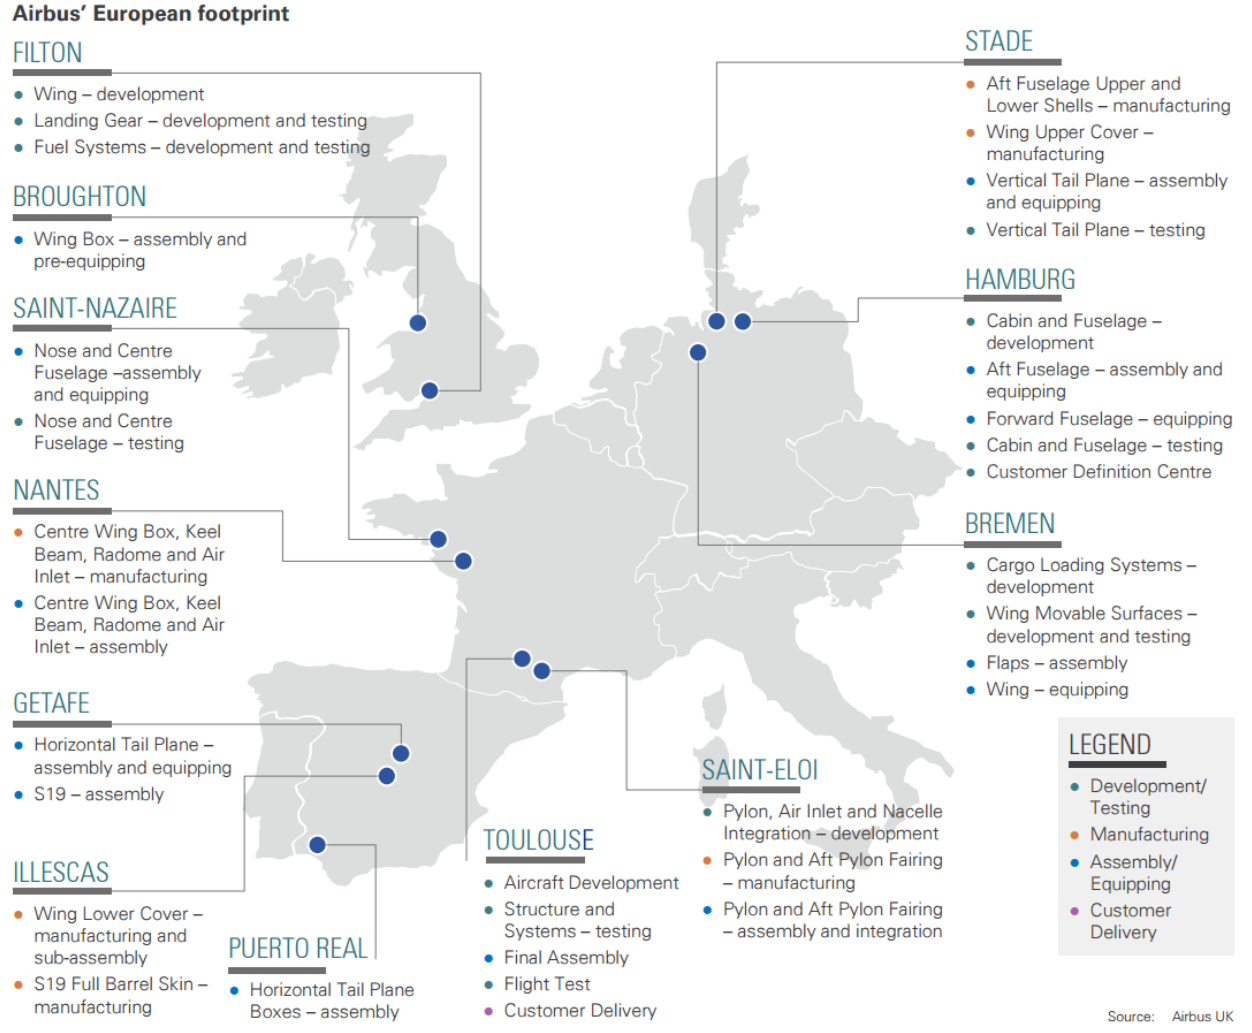
\includegraphics[width=120mm,scale=1]{figs/Airbus-1}
	\caption{Integrated Supply Chains \cite{Airbus:ADS}}
	\label{fig:Airbus} 
\end{figure} 
%\clearpage

Blockchains can offer numerous benefits for streamlining processes and increasing transparency across the supply chain. Coupled with Smart Contracts and IoT, supply chain can become one of the killer applications of the blockchain. Smart Contract platforms such as the Ethereum can use tracking data to automate various functions and events in the supply chain life cycle. Ethereum’s distributed ledger also provides total transparency to all parties involved. By increasing automation within supply chain processes they can reduce complexity and eliminate errors and delays. Some of the key benefit of blockchains in the context of SCM are follows:

\textbf{Transparency:}
Its shared ledger enables all stakeholders to have the same view of the data stored on the blockchain. Transparency is greatly increased due to everyone having real time access to the same data.

\textbf{Traceability and Compliance:}
Every transaction recorded on the blockchain is cryptographically verified. This increases traceability, reduces fraud, and helps to increase compliance for existing products. 

\textbf{Security:}
Any system built on the blockchain is by design highly secure against DDoS attacks and single points of failure. Each transaction on the blockchain is replicated across multiple nodes on a distributed ledger. Each block links to a previous block hence any attacker wanting to modify data in any block will need to modify all subsequent blocks as well.

\textbf{Trust:}
Most traditional Supply Chain Management(SCM) systems allow participants a very limited view throughout the supply chain life cycle. Usually participants only have access to information necessary to successfully realize the next process of the supply chain. This creates information asymmetry between different stake holders. Decentralized blockchain based SCM systems can allow participants to have same view of the entire system and hence reduce information asymmetry and increase trust.
\clearpage
%check motivation again see if i have said that blockchain icnreases trust or allows participants to trust data from untrusted sources, reduces complexity, etc

\subsection{Thesis Objective}
The primary goal of this thesis is to design and develop a secure decentralized supply chain management and shipment tracking system. The backbone for this system will be a Smart Contract for monitoring and regulating supply chain cycles under strict conditions. Two types of decentralized applications will be developed for interacting with the Smart Contract. In order to realize this system following questions and issues must be addressed:

\begin{enumerate}[label=(\alph*)]
\item Which blockchain platform is best suited for development of this system? 
\item How to reduce complexity and increase automation in supply chain processes?
\item Provide real time access to critical information for all relevant stake holders.
\item Enhance the blockchain security model by using Post Quantum Primitives.
\end{enumerate}

The design and requirements of this system are based on a use case scenario presented in chapter \ref{usecase}. 

%check motivation again see if i have said that blockchain icnreases trust or allows participants to trust data from untrusted sources, reduces complexity, etc. Add these as research objectives for our system. I.e. greatly increase trust, provide real time insight into critical data like violation events or some other important event, increase automation. sub questions could be whihc blockchain platform is most useful etc.
%Increase trust in SCM and Information, How to increase trust by using blockchains

\section{Blockchain: Technical Primer} \label{Blockchain}
This chapter explains some of the technical concepts and terminologies related to blockchain. This technology allows participants to transact with each other using a peer-to-peer network that guarantees censorship resistance, immutability, transaction finality, and protection against double spend attacks. In order to better explain how it works consider figure [\ref{fig:bc-workflow}]. Alice wants to transfer two bitcoins to Bob. She uses her private key to creates a signed transaction for transferring these coins to Bob. Every user in the network has pair of keys; a public key that serves as their unique identifier or address and a private key for signing transactions see section [\ref{AC}]. The signed transaction is broadcast to the bitcoin network where it waits until it is picked up by a special node called a miner. The miner verifies transaction signatures and batches pending transactions into blocks. Each block carries the hash of the one that came immediately before it. Next step is to calculate the hash of the entire block and append it at the end of the blockchain see figure [\ref{fig:bc-workflow}]. Blockchain protocols have built in consensus mechanism to ensure that peers always agree on only one longest chain see section [\ref{Mining}]. Blockchain is not just a technology it is actually a systems and like most systems it is composed of individual components which come together to make the whole. The next few sections explain the important building blocks or sub components of the blockchain system.

\begin{figure}[t]
	\centering
    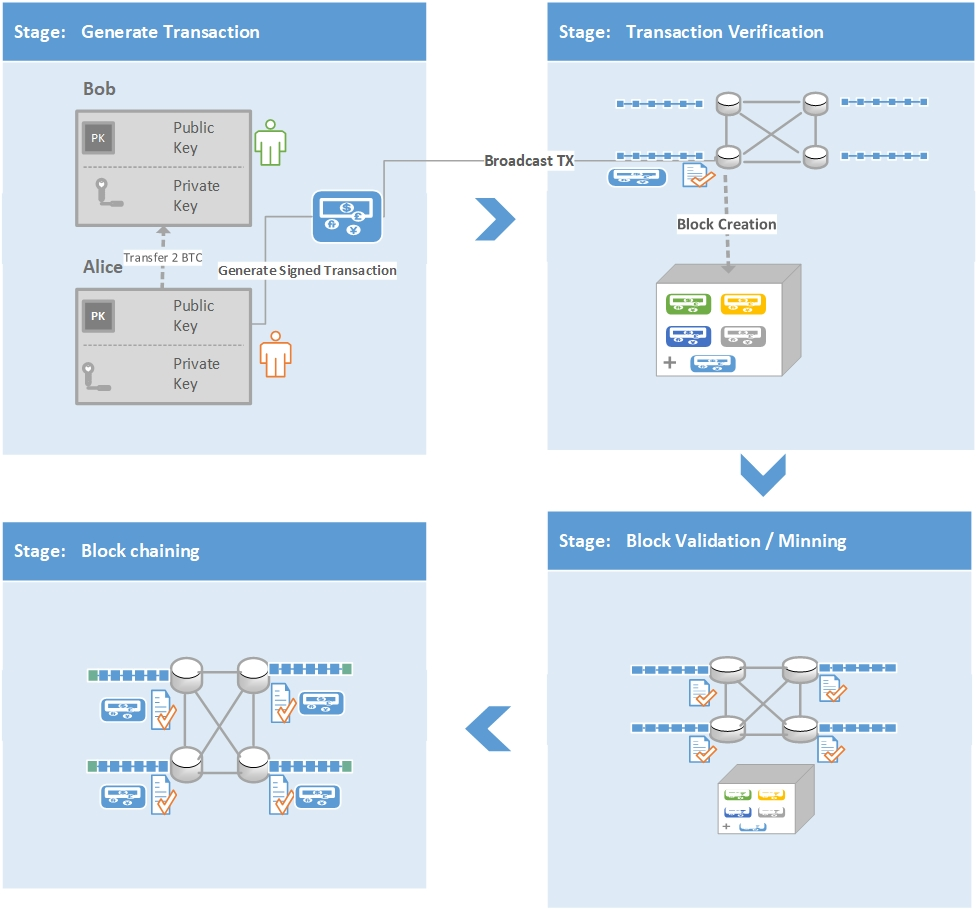
\includegraphics[width=160mm,scale=1]{figs/bc-workflow}
	\caption{How does blockchain work?}
	\label{fig:bc-workflow}
\end{figure}
\clearpage

\subsection{Distributed Ledger Technology} 
Distributed ledger Technology refers to a shared and distributed database replicated across members of a peer-to-peer network. Each member of the network receives the same copy of the data. New data can only be added to the ledger when consensus is achieved among the members. Consensus rules and mechanisms [\ref{Mining}] may vary from network to network. These rules are designed to ensure that data on the ledger remains synchronized across network participants. Blockchain is a special type of distributed ledger where cryptography is used to achieve consensus and ensure transaction authenticity.  Information stored on the blockchain is immutable i.e. once recorded it cannot be altered. Blockchain is not the only structure used for DLT. IOTA \cite{wiki:003} and Hashgraph have successfully employed Directed Acyclic Graphs (DAG) \cite{wiki:002} for creating their DLT. 
\subsection{Asymmetric Cryptography} \label{AC}
Asymmetric or public key cryptography is an important building block of any blockchain network. This cryptography technique relies on a pair of keys: A public key which is widely available or shared with everyone, and a private key which is only known to the owner. These two keys are mathetimatically related to each other in that one key usually encrypts and the other key is used for decryption. If the private key encrypts only the corresponding public key can decrypt and vice versa \cite{wiki:004}. Public key cryptography is widely employed for:

\textbf{Public key Encryption:} is an encryption technique where data is encrypted using senders public key. The recipient can only decrypt the data and read the message if he is in possession of the corresponding private key.

\textbf{Digital Signatures:} based on public key cryptography are used in a number of applications including blockchain. Data or message is signed with sender’s private key. Anyone can verify the message signature using the corresponding public key. In Bitcoin, Ethereum and other blockchain networks digital signatures are used to guarantee authenticity, integrity and non-repudiation.
\subsubsection{Digital Wallets}
In cryptocurrency applications we often hear the term digital wallets. It is a program which shows users account balance and helps them transfer coins to other users. In essence a digital wallet is the private key of that user. It provides additional functionalities like signing transactions for transferring coins, and querying the blockchain to get the cryptocurrency balance associated with their private key.  Figure [\ref{fig:bc-sig}] shows how digital signatures are used in the blockchain. 

\begin{figure}[h]
	\centering
    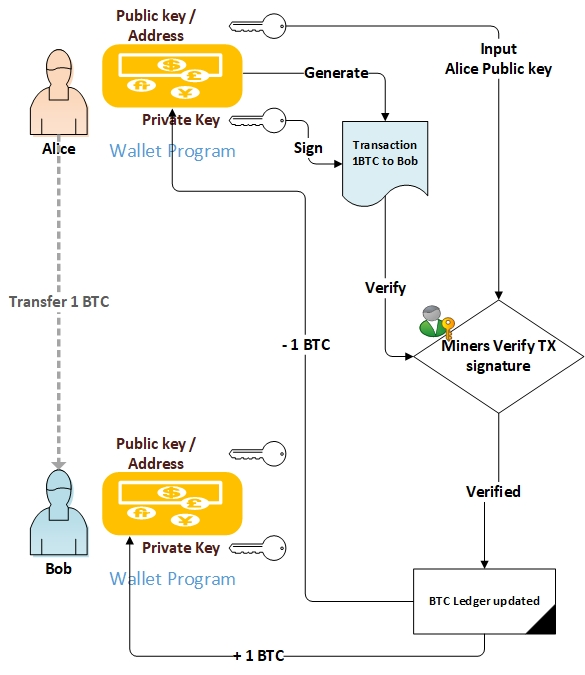
\includegraphics[width=160mm,scale=1]{figs/sig}
	\caption{Digital Signatures in Blockchain}
	\label{fig:bc-sig}
\end{figure}
\clearpage

\subsection{Hashing}
Hashing is used to calculate fixed length hashes for variable length data. Hashing algorithms are designed in a way that even a slight change in the input data will result in a vastly different output hash. All cryptocurrency networks use some sort of hashing algorithms in their mining [\ref{Mining}] process. Ethereum uses an algorithm called Ethash (modfied Dagger Hashimoto) and bitcoin uses SHA-256 \cite{dang_2015} hashing algorithm. These algorithms are used as a mechanism to guarantee integrity and to prevent unauthorized tampering and corruption of the distributed ledger. They are used to link blocks with each other in the blockchain. Each new block contains the hash of the blockchain that came before it as shown in figure [\ref{fig:blockchain}]. Each blocks hash represents the state of the blockchain when it was created. This allows anyone to easily verify the complete state of the entire blockchain. Any attempt to alter data in any block will result in a vastly different hash for that block and will also require that hashes for all subsequent blocks be recalculated.
\subsection{Merkle Trees}
Blockchain is defined as a continuously growing list of transactions called blocks \cite{wiki:001}. A block contains multiple transactions and a hash as shown in figure [\ref{fig:blockchain}]. This hash is calculated over the entire block. A block is actually a special data structure which is implemented with the help of a Merkle tree as shown in figure [\ref{fig:blockdisected}]. Andreas Antonopoulos defines merkle trees in his book “Mastering Bitcoin” as \textit{“A merkle tree, also known as a binary hash tree, is a data structure used for efficiently summarizing and verifying the integrity of large sets of data.”} \cite{andy_mb} (ch.9). They are used to summarize all transactions in a block using cryptographic hashes. This enables fast and efficient verification of any transaction in a particular block. In a tree comprising of N data elements only \(2*log2 (N)\) calculations are required to verify if a particular data element or transaction is included or not. Without Merkle trees it will be prohibitively expensive to run blockchain nodes which would severely impact the decentralization of the system. 
In bitcoin a Merkle tree is constructed by recursively hashing pair of nodes using SHA256 cryptographic hash function as shown in figure [\ref{fig:mtree}] \cite{andy_mb} (ch.9).  In the example tree there are four leaf nodes storing hashes of four transactions. The leaf nodes do not store actual transactions rather TX data is hashed and result is stored in the Merkle tree. Each leaf node is designated as \( H_{A}, H_{B}, H_{C}, H_{D} \) and given by the equation: \[ H_{A} = SHA256(SHA256(Transaction_{A}))\]
Since Merkle trees are in essence binary trees hence even number of nodes are required to have a balanced tree. Two leaf nodes are hashed together to form a parent node as given by equation \eqref{eq:2}. In the event of odd number of transactions, the last transaction is duplicated to have an even number of leaf nodes equation \eqref{eq:3}. The recursive hashing process starts from the bottom and continues until there is only one node left at the top which is called the Merkle Root. This is the parent hash of all child nodes and summarizes all the data in all transactions. The root hash is placed in the block header.
\begin{equation}
  \label{eq:2}
H_{AB} = SHA256(SHA256(H_{A} + H_{B}))
\end{equation}

\begin{equation}
  \label{eq:3}
 H_{CC} = SHA256(SHA256(H_{C} + H_{C}))
\end{equation}


\begin{figure}[h]
	\centering
    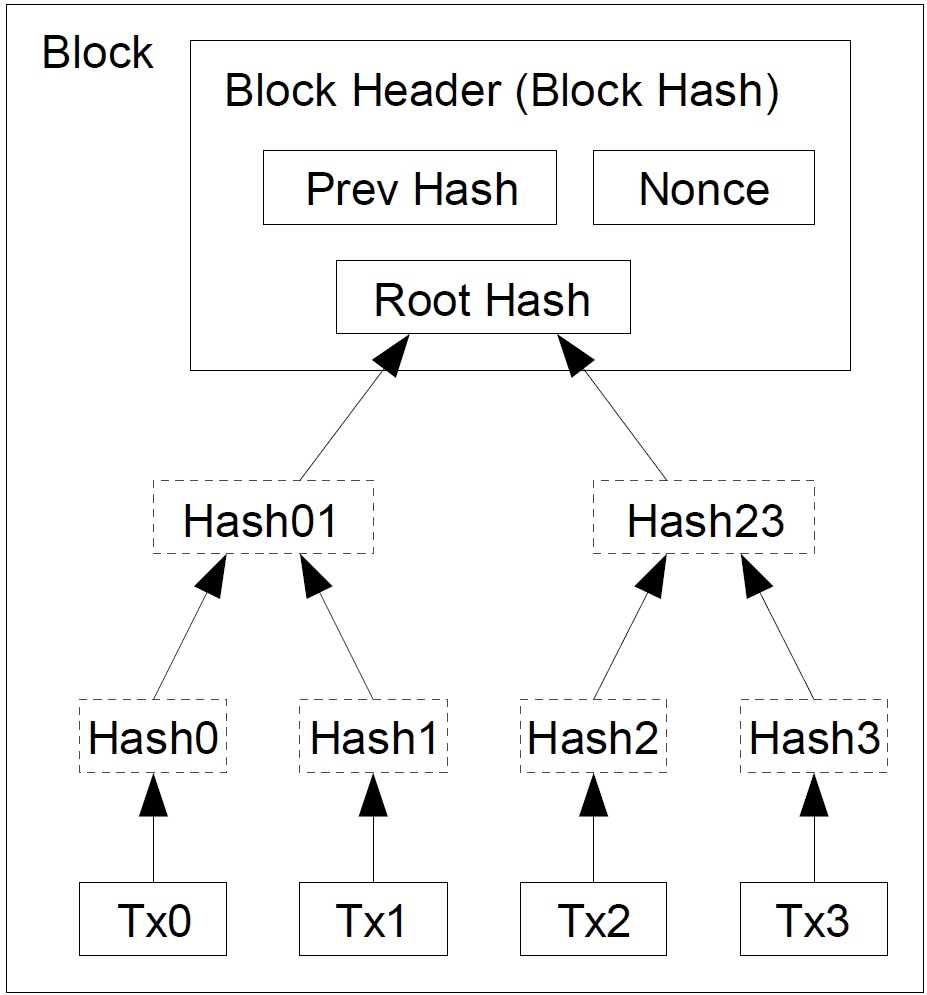
\includegraphics[width=120mm,scale=0.5]{figs/blockdisected}
	\caption{Transactions Hashed in a Merkle Tree \cite{paper:001}}
	\label{fig:blockdisected}
\end{figure}
\begin{figure}[h]
	\centering
    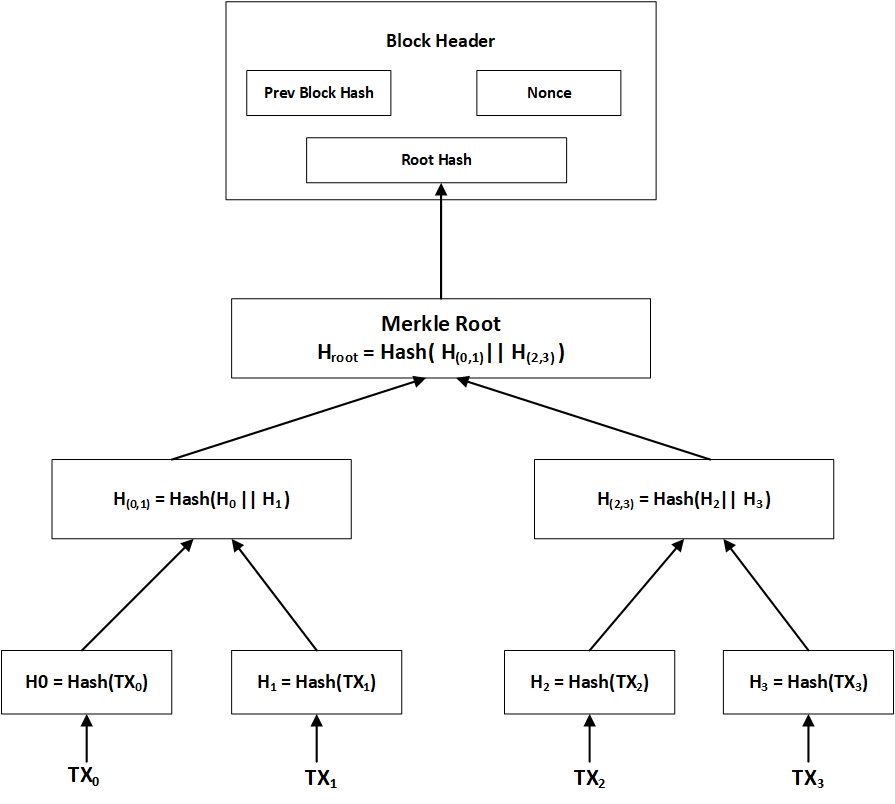
\includegraphics[width=160mm,scale=0.5]{figs/mtree}
	\caption{Constructing a Merkle Tree, adapted from \cite{andy_mb}}
	\label{fig:mtree}
\end{figure}
\clearpage

\subsection{Consensus Mechanisms - Mining} \label{Mining}
Electronic coins are defined as a chain of digital signatures that serves to establish ownership. In order for Alice to transfer one coin to Bob she must sign the hash of a previous transaction and the public key of the next owner i.e. Bob. Anyone can verify the chain of ownership by verifying signatures. This process only verifies that Alice was in possession of the coin at some point in time, it does not guarantee that Alice did not try to spend the same coin more than once.  Therefor a mechanism is needed that guarantees that any previous owner (Alice) did not sign any earlier transaction for transferring the same coin. The only way to verify this in a decentralize system is to announce all transactions and to have a mechanism to ensure that all participants agree on a single shared history or order of transactions. Payee (Bob) needs proof that at the time of each transaction, the majority of participants agreed that it was the first one \cite{paper:001}. The process which establishes consensus among all participants is called Mining.
%%%%%%%%%%%%%%%%%%%%%%Extras%%%%%%%%%%%%%%%%%%%%%%%%%
%put the figure of digital coin from bitcoin white paper section transactions
\subsubsection{Mining}
Mining underpins bitcoin or blockchain’s security model. This process is a designed to guarantee security and integrity of the distributed ledger. It serves to protect the network from fraudulent transactions and double spend attacks i.e. spending the same coins twice. It is also the process by which new blocks are generated. Miners spend something of value like electricity in the form of computing power by running complicated algorithms (Proof of Work). They are rewarded by the network with block rewards or newly minted coins. It prevents bad actors or attackers from modifying the state of decentralized ledger against network rules. Attackers will need to control at least fifty-one percent of network hash rate to mount a successful attack. This is virtually impossible in a sufficiently decentralized network like Bitcoin or Ethereum. There are two main type of mining algorithms Proof-of-Work \ref{PW} and Proof-of-Stake \ref{PS}.
  
\subsubsection{Proof-of-Work} \label{PW}
It was proposed by Satoshi Nakamoto in the bitcoin white paper \cite{paper:001}as means for establishing consensus. Miners solve complicated mathematical problems to validate transactions. Pending transactions are batched into blocks and the miners compete with each other to calculate the hash of the block. The hash output of the block must start with specific number of leading zeroes in order to satisfy protocol rules. The exact number of leading zeroes depend upon the network difficulty and is adjusted automatically every 2016 block. This difficulty determines how easy or hard it is to find the output hash for a block. The function that calculates difficulty is determined by a moving average and targets average number of blocks per hour. If blocks are generated too fast, the difficulty increases and vice versa. This is done in order to compensate for increasing hardware speed and varying interests in running nodes. Proof-of-work protocols can be summarized in the following steps \cite{medium:001}.

\begin{itemize}
  \item Miners try to find the hash output for a block with a fixed number of leading zeroes. They do this by repeatedly changing part of the block called nonce and recalculating the hash output.
  \item First miner to solve the puzzle and find the hash broadcasts his solution or proof-of-work to the rest of the network.
  \item Upon receiving the solution other miners verify it to ensure that it is correct. Before they agree to add the it to the blockchain they verify all the transaction in the block to make sure they are valid.
  \item If majority of miners agree on the solution and agree to add the block to the blockchain than consensus is achieved.
\end{itemize}

\subsubsection{Proof-of-Stake} \label{PS}
Proof of Work algorithms require miners to solve complicated math problems to verify transactions and generate new blocks. This approach has some inherent disadvantages. It requires huge amounts of electricity to achieve consensus in large blockchain networks such as Bitcoin and Ethereum. Some estimates have put bitcoins annual energy consumption on the same level as countries likes Austria or Switzerland. POW operates on the basis of one CPU one vote model. This approach can lead to mining centralization by large mining pools and chip manufacturers. Proof of Stake is an alternative approach for reaching consensus and protecting from double spend attacks in a decentralized network. It solves many problems inherent to POW algorithms. It is defined as \textit{“Proof of Stake (PoS) is a category of consensus algorithms for public blockchains that depend on a validator's economic stake in the network”} \cite{ethwiki:006}. POS requires users or forgers as they are called to lock up their digital coins in an escrow to get a chance to validate new blocks. The deposited coins serve as collateral and an incentive for the forgers to behave honestly. If a forger approves fraudulent transaction they will lose the coins they staked and will be banned from participating in the block validation process in the future. The crux of POS systems is the fact that for any attack to be successful the attacker will need to own majority of the coins on the network. Therefore, the attacker will be the one most severely impacted by his own attack \cite{bitwiki:005}. This serves as a huge deterrent against any potential bad actors. Block validators are incentivized with block rewards (combination of Tx fees and coins). They are selected by the network in a pseudo – random selection process based on a combination of factors. Selecting forgers solely on the size of their stake will hugely benefit the rich miners making the rich even more richer. There are several methods to avoid these problems two of which are given below. \cite{medium:002}\cite{misc:001}

\textbf{Coin Age based Selection:}
This method choses validators based on how long their coins have been staked for or the ‘coin age’ of their stake. The coin age is calculated by multiplying the size of a validators stake with the number of days the coins have been held in escrow. Once a validator generates a block their coin age is reset and they have to wait a fixed amount of time before they can be selected to validate another block \cite{misc:001}.

\textbf{Randomized Block Selection:}
This method choses validators based on a combination of lowest hash value and the size of their stake \cite{misc:001}.

%%%%%%%%%%%%%%%%%%%%%%Extras%%%%%%%%%%%%%%%%%%%%%%%%%
%\subsubsection{Delegated Proof of stake}
%\subsection{Full Nodes}
%\subsection{Transaction Finality}
%mention how finality can impact confirmation times and how it might impact any %potential supply chain management app.
%https://medium.com/coinmonks/blockchain-finality-pow-and-pos-35915a37c682
\subsection{Challenges:Scaling Debate}\label{scaling}
Blockchain technology is still in its infancy. It is a novel idea to solve several interesting problems in a trustless and decentralized manner, however in order to compete with existing centralized platforms it needs to be able to scale to handle millions of transactions per second. Let us consider the most common use case where the blockchain is used for making payments or to transfer assets between users. Bitcoin can on average perform 3 to 4 transactions per second while Ethereum can handle up to 20 transactions per second. Compare this to Visa which on average handled over 1100 transactions per second in 2016 and has an estimated capacity to perform up to 100000 transactions in a second \cite{medium:003}. Transaction speed measured in TPS is an important to metric to measure the performance of any financial system. During 2016 and 2017 major blockchain networks saw enormous growth in their user base. This caused exponential increase in transaction volume resulting in congested networks which caused huge delays in transaction confirmations [\ref{fig:mct}]. This had a domino effect on transaction fees as well, causing them to sky rocket as miners are incentivized to pick transactions with higher fees to mine first. The long confirmation delays coupled with high transactions fees caused many organizations and vendors to stop accepting bitcoins. There was an interesting case in 2017 when a conference held to promote the benefits of bitcoin and blockchain stopped accepting bitcoins as a mode of payment due precisely due to reasons outlined earlier.  The scaling problem is further amplified in smart contract platforms like Ethereum[\ref{eth}] which aim to be a hub for large scale decentralized applications or Dapps. Most existing and proposed Dapps use mircotransaction (MTX) as part of their business model. “Microtransactions are a business model where users can purchase virtual goods via micropayments” \cite{wiki:007}. In order to efficiently run such applications Ethereum needs a way to effectively handle $\mu$-transactions. In most cases these transactions need to be executed immediately and cannot wait for long block confirmation times. According to some estimates using current mechanisms “we’re roughly 250x off being able to run a 10m user app and 25,000x off being able to run Facebook on chain” \cite{medium:003}.  This requires exponential increase in transactions per second for blockchain to become a viable alternative to centralized solutions.
\begin{figure}[h]
	\centering
    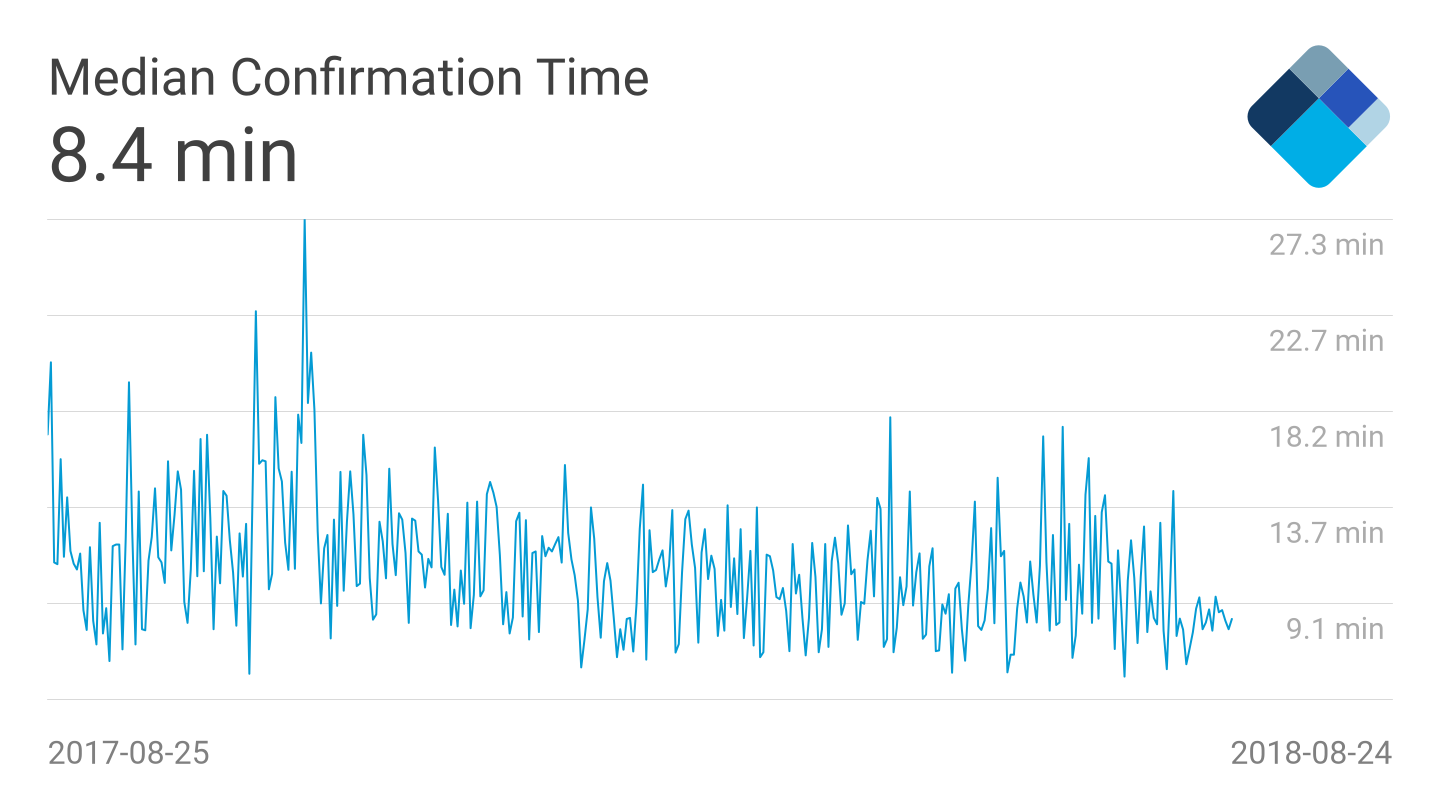
\includegraphics[width=120mm,scale=1]{figs/median-confirmation-time}
	\caption{Median confirmation times for BTC transactions \cite{fig:001}}
	\label{fig:mct}
\end{figure}
\clearpage

\subsubsection{Increasing Blocksize}
Transactions are grouped into blocks before they are verified. POW consensus rules require that there is some distance between successive blocks so that each verified block is successively incorporated by a majority of nodes in their copy of the ledger. This means that roughly only one block is generated every ten minutes \cite{paper:001}. In addition, some blockchains like Bitcoin have placed an upper limit on the size of each block. Currently for bitcoin the block size limit is 1 megabyte. One suggestion is to simply increase the block limit to allow more transactions to be verified at any given time.  This solution however has many problems first of all increasing block size results in only a linear increase in transactions per second. Secondly, it will adversely impact the decentralization of the network. Larger blocks require higher computational power to process each block and also drastically impact the size of the distributed ledger. This leads to more centralization as not everyone can afford the equipment required to successfully mine new blocks \cite{medium:006}. 
\subsubsection{Payment Channels - Lightning Network}
An alternative solution is to use Layer - 2 transaction networks. Lightning network is bitcoins proposed solution for the scaling problem. Lightning network is defined as \textit{“A decentralized system for instant, high-volume micropayments that removes the risk of delegating custody of funds to trusted third parties”} \cite{paper:002}. It advocates using payment channels to handle transactions off chain. \textit{“Payment Channel is class of techniques designed to allow users to make multiple Bitcoin transactions without committing all of the transactions to the Bitcoin block chain. In a typical payment channel, only two transactions are added to the block chain but an unlimited or nearly unlimited number of payments can be made between the participants”} \cite{bitwiki:006}.  Payment channels are essentially multi-signature bitcoin addresses. In order to spend funds from the channel both parties must sign off on the transaction agreeing to the new balance of the channel. The new balance is stored as the most recent transaction in the channel. Simply put, a payment channel is a smart contract on the bitcoin blockchain which is mostly executed off-chain after creation. In an ideal case, the only two transactions that go on the block chain are the ones for opening and closing a channel \cite{misc:011}. Participants of the channels can make unlimited instant transactions to each other while the channel is open. \textit{“Security is enforced by blockchain smart-contracts without creating an on-blockchain transaction for individual payments. Payment speed is measured in milliseconds to seconds”} \cite{paper:002}. This enables users to make off chain payments with confidence. If anything goes wrong blockchain can cryptographically verify the terms of the smart contract and enforce them on-chain \cite{bitwiki:006} \cite{misc:012}.
\clearpage
\subsubsection{Sidechains}
Sidechain is a blockchain that runs parallel to the main blockchain. It extends the functionality of the main chain enabling decentralize transfer of assets and tokens between the two chains. They allow coins to be moved between two separate blockchains. Tokens from the main chain can be securely moved to the sidechain and used in these chains. The token transfer takes places at a fixed predetermined rate \cite{misc:013}. In order to transfer main chain assets to a side chain they are sent to a special address on the main chain. Once this transaction is verified a confirmation is broadcast in the sidechain enabling the network to assign equivalent assets to the users account in the sidechain \cite{paper:004}. They can help with blockchain scaling as they can take some of the pressure of the main chain. Developers can design specialized sidechains to run their Dapps more efficiently while still taking advantage of security and decentralization provided by the mainchain. Sidechains are implemented using a Two – way peg as shown in figure [\ref{fig:SC}].
\vspace*{2cm}
\begin{figure}[h]
	\centering
    \includegraphics[width=160mm,scale=1]{figs/sidechain}
	\caption{Two way Pegged Sidechain }
	\label{fig:SC}
\end{figure}

\textbf{RootStock RSK SideChain}
It is a sidechain to bitcoin. It is Two-way pegged to bitcoin. RSK code aims to be backwards compatible to Ethereum i.e. code can be written in solidity or serpent and can be used on Ethereum. RSK aims to be a platform for decentralized applications and smart contracts on bitcoin. Miners are incentivized to mine smart contracts on RSK by rewarding them with bitcoins. Bitcoin miners can simultaneously mine both blockchains and rewarded through a process called “merge-mining”. Rootstock has its own version of Ethereum virtual machine (EVM). Currently the developers are working on what is called a federated peg which is essentially a system of notaries and a Multisignature exit address. The developers aim to go from federated peg to a two-way pegged system based on Simplified Payment Verification (SPV) \cite{andy_mb} \cite{paper:005}. 

\textbf{Federated peg:} is a system consisting of a set of notaries and a Multisignature exit address. When you send funds to this exit address you can create an SPV proof on RSK sidechain. This SPV proof allows you to convert the locked bitcoins in the federated address into bitcoins on rootstock sidechain. This is done automatically. However, moving funds from RSK back to bitcoin requires collaboration of federators. Basically a smart contract acts as bridge master and controls all unspent transaction outputs. This contract broadcasts a transaction to federators by using a log message. On receiving this message, federators send signatures to bridge master who combines all these signatures in to a fully signed transaction. This signed transaction is broadcast to RSK blockchain where any user can put this transaction onto bitcoin blockchain. This unlocks bitcoins on the bitcoin blockchain \cite{paper:005}.



%May be rename this chapter as State of the Art
\section{Blockchain Applications}
Companies and People across the globe are exploring applications of blockchain technology across several industries. This chapter details blockchain applications and projects from various sectors including finance, Internet of Things, Supply chain Management and File hosting and sharing. 
\subsection{Crypto Currencies}
Bitcoin was the first ever application of blockchain technology. It was proposed and developed shortly after the financial crash of 2007. This crash was caused by the irregularities in the existing centralized financial institutions and banks. The biggest problem with traditional banking is that it centralizes trust in a few large financial institutions and banks. This system works only as long as these banks operate reliably and responsibly. The financial crash of 2007 showed that they cannot be always trusted to act responsibly \cite{misc:009}. Bitcoin was developed to address problems prevalent in existing centralized financial system. It solves these problems by developing a system which removes all central entities and trust is established through a system of checks and balances [\ref{Blockchain}]. Cryptocurrency sector experienced huge growth in terms of users and investment during 2016 and 2017 and at one point was worth close to 500 billion dollars \cite{misc:010}. Unfortunately, most of this growth was due to speculative investments and has not yet translated into large scale adoption of Cryptocurrencies in everyday business and finance. Blockchain powered financial systems have huge promise provided they are able to solve some of the challenges outlined in section \ref{scaling}.
\subsection{Internet of Things}
IoT is the next wave of automation promising to disrupt industrial and domestic structures and processes. The billions of smart devices coming online could transform homes, cities, offices and factory floors \cite{misc:008}. \textit{“IoT holds the promise to expand business processes and to accelerate growth. However, the rapid evolution of the IoT market has caused an explosion in the number and variety of IoT solutions, which created real challenges as the industry evolves, mainly, the urgent need for a secure IoT model to perform common tasks such as sensing, processing, storage, and communicating”} \cite{misc:002}. Currently IoT ecosystems are realized using brokered communication models based on client/server paradigm. Devices are connected through cloud servers using the internet even if they are few feet away from each other. Further more centralized models struggle to scale up to meet the demands of billions of users or devices \cite{misc:004}. Blockchains offer an intriguing alternative as a secure and decentralized IoT command, control and communication model. Blockchain and Smart contract based solutions should be more manageable and scalable then traditional ones. Blockchains are inherently tamper resistant hence they will prevent one or more rogue devices from causing a complete system breakdown across a home, factory, or transportation system. Blockchain in IoT sphere has the potential to revolutionize several industries and businesses \cite{misc:008}, \cite{misc:004}, \cite{misc:002}. There are several exciting projects working towards this goal. Sections \ref{Adept} and \ref{Filament} describe two projects at the forefront of blockchain and IoT.



%\textbf{Smart Washing Machine}
%This example is a realization of proof of concept proposal from Samsung. \textit{“Imagine a washer that autonomously contacts suppliers and places orders when it’s low on detergent, performs self-service and maintenance, downloads new washing programs from outside sources, schedules its cycles to take advantage of electricity prices and negotiates with peer devices to optimize its environment”} \cite{misc:004}. If the machine is connected to some sort of ledger be it private or public, it can automatically pay the detergent suppliers and repairmen \cite{misc:004} \cite{misc:005}.

\subsubsection{Autonomous Decentralized Peer-to-Peer Telemetry (ADEPT)} \label{Adept}
ADEPT is a joint venture between IBM and Samsung Electronics. It is developed to serve as a validation platform for projects proposing to connect IoT and Blockchain. It envisions network of devices that are capable of autonomously maintaining themselves. Adept is working towards integrating IBMs Watson IoT platform with blockchain technologies. This project is still in development stage but proof of concept has already been implemented \cite{misc:005}. It uses blockchains as the backbone of the system using a mix of proof of work and proof stake to secure transactions. The ADEPT architecture supports three foundational functions.
\begin{itemize}
  \item Peer to Peer encrypted messaging using a secure messaging protocol called TELEHASh \cite{misc:005}.
  \item Decentralized file sharing based on BitTorrent protocol \cite{misc:005}.
\item Decentralize device coordination and control
In the absence of centralize controller, device control and coordination becomes significantly challenging. Adept uses Ethereum or hyper ledger blockchain to implement this in a trustless secure fashion \cite{misc:005}.

\end{itemize}
Ultimately it will enable IoT devices to send data to private blockchain ledgers for inclusion in shared transactions with tamper-resistant records. Devices will be able to communicate with the blockchain in order to update or validate smart contracts. This will improve transparency and reduce conflicts by empowering all stake holders. Each stakeholder will have access to the same data and could easily verify all transactions \cite{misc:005}, \cite{misc:004}. 
%\clearpage

\subsubsection{Filament} \label{Filament}
Filament is a technology stack that \textit{“enables devices to discover, communicate, and interact with each other in a fully autonomous and distributed manner”} \cite{misc:006}. Its main focus is industrial Internet of Things. \textit{“The Filament technology stack is built upon five key principles: Security, Privacy, Autonomy, Decentralization, and Exchange (SPADE)”} \cite{misc:006}. Filament uses Telehash for secure encrypted device to device communication. Secure Identity is provided by blockchain. Once a secure communication channel has been established between devices, smart contracts are used to interact with them, or to enable them to transact with each other. Smart Contracts in Filament run directly on device and accept or run transactions from other devices based on contractual terms. It uses a protocol suite called “JOSE” (Javascript Object signing and Encryption) to implement smart contracts on the devices \cite{misc:007}. In order to enable micro transactions on these embedded devices authors of the Filament project propose a solution called Penny Bank. It allows the devices to exchange small amounts of value with each other without involving the blockchain for every single transaction thereby avoiding heavy transaction fees \cite{misc:006}.

\subsection{Supply Chain Management}
Blockchains allow secure and permanent documentation of transactions in a decentralized ledger. They can be transparently monitored by all parties. This can improve efficiency and reduce human mistakes and delays. It can also enable users to verify authenticity of products by tracking them from their origin. An example of this is securing supply chains of diamonds from mine to consumers. IBM’s Hyperledger Fabric is one of the proposals working in this field. It is permissioned blockchain infrastructure designed specifically for handling supply chain management tasks. Using blockchain technologies customers can verify when and where a diamond was mined, all the places it passed through during its journey to the retailer, and whether or not during any step of the supply chain it crossed any moral or legal grey areas i.e. if it’s a blood diamond \cite{misc:014}.
\subsubsection{Skuchain}
Sku chain is a platform that uses blockchain to provide security, efficiency and transparency to supply chains. Today’s supply chain management tools such as ERP systems, Inventory Management systems, Letters of credits, Purchase and Invoicing tools have significant friction and problems interfacing with each other. This results in increased costs and delays in every process of the supply chain. Skuchain proposes tools in order to resolve some of these issues \cite{misc:015}.

\textbf{IMT:}
\textit{“IMT provides inventory financing that de-risks transactions and unlocks capital opportunities for the entire supply chain. The original contract between the buyer and seller is assigned to IMT in the blockchain. This acts as a Blockchain Based Security Interest that provides the collateral to an investor in the IMT fund. IMT uses its funds to purchase goods from the seller and stores them at a VMI warehouse. Finished goods are shipped pursuant to a purchase order from the buyer, a process covered by insurance. The buyer then pays IMT for the goods”} \cite{misc:015}.

\textbf{Brackets:}
Smart contracts on the skuchain are called brackets. They are cryptographically secured. They provide some key advantages. 

\begin{itemize}

\item They are designed to release collateral as a result of being triggered automatically by real world events \cite{misc:015}. 
\item  They improve transparency for all participants by providing real time view of transaction state \cite{misc:015}. 
\item  \textit{“It enhances liquidity of collateralized assets in a supply chain by improving upon current trade finance instruments such as Factoring, PO Financing and Vendor Managed Inventory Financing. It also creates the opportunity for Deep Tier Financing”} \cite{misc:015}. 
\end{itemize}

\textbf{PopCodes:}
\textit{“Popcodes are Proof of Provenance codes, a crypto-serialization solution to track flow of goods on SKU level. They provide bank-grade traceability to track physical value in the supply chain. Popcodes are sophisticated in their ability to track sub-assemblies, parts and raw materials used to make a finished product. Using Popcodes, an enterprise can gain JIT visibility across the entire supply chain ecosystem, enabling optimal agility and planning. It also provides end-consumer visibility into the entire history of the product”} \cite{misc:015}.

\subsubsection{Provenance}
This project is working on using blockchain technology to enable secure traceability of certifications and other salient information in the supply chain. It aims to become a platform for verifying authenticity of goods. \textit{“Provenance enables every physical product to come with a digital ‘passport’ that proves authenticity (Is this product what it claims to be?) and origin (Where does this product come from?), creating an auditable record of the journey behind all physical products”} \cite{paper:006}. They are creating a decentralized app for solving certification and chain of custody challenge in sustainable supply chains. It proposes a system to assign and verify certain properties of physical products using the blockchain. There are six different actors involved in the proposed scheme namely.
\begin{itemize}
\item Producers 
\item Manufacturers
\item Registrars, they provide unique identity to other actors in the scheme 
\item Standards organizations, which define the rules of a certain scheme (e.g., Fairtrade) 
\item Certifiers and auditors 
\item Customers
 
\end{itemize}
The architecture in their white paper \cite{paper:006} consists of number of modular programs. Namely Registration program, Standards programs, Production programs, and Manufacturing programs. Each contract is deployed on the blockchain independently but since all of them work within the same blockchain system they can interact without friction. Technologies such as NFC, RFID, barcodes, and digital tags link physical products to their digital representation on the blockchain. Furthermore, user facing application in the form of smart phone applications will facilitate access to the blockchain. They will aggregate and display information to customers in real time, detailing every step of the supply chain \cite{paper:006}.

\subsection{Filesharing}
Filecoin, SiaCoin and Storj are some of the proposals for creating a decentralized platform for filesharing, storage and cloud computing using the blockchain. The idea is simple users instead of uploading files to a central cloud server hosted at google, Microsoft or Dropbox files are shredded, encrypted and spread across the distributed file storage network based on the blockchain. Only the uploader holds the keys to call smart contracts to decrypt and reassemble the files. People participating as hosts in the network rent out their storage spaces and get paid in return for the services they provide \cite{misc:016}.
\subsubsection{FileCoin}
\textbf{Filecoin}
\textit{ “Filecoin is a decentralized storage network that is auditable and publically verifiable. Clients pay miners for data storage and retrieval. Clients offer data storage and disk space in exchange for payments. The network achieves robustness by replicating and dispersing content while automatically detecting and repairing replica failures”} \cite{paper:007}.

\textbf{Proof of Storage}
Proof of storage is a class of decentralized challenge response protocols. They allow a storage provider or host to efficiently verify the integrity of the data stored on their device to their users or clients. The client sends encrypted version of its data to the hosting node for storage, while keeping a small portion of that data himself so he can cryptographically verify the integrity of data stored on the hosting node at any time \cite{paper:007}.

\textbf{Proof of Replication}
\textbf{Proof of Replication}
Filecoin introduced a special form of proof of storage protocols called Proof of Replication. It is an extension of Proof of Storage protocol. It enables a miner to convince a user that some data D has been successfully replicated to its own unique physical storage S. It uses challenge/ response protocol to achieve this \cite{paper:007}. Traditional PoS protocols are limited in that they only prove that a miner or host was in possession of data at the time of challenge/response. Filecoin developed PoR protocol in order to provide stronger guarantees against Sybil attacks, Outsourcing attacks and Generation attacks \cite{paper:007}. These attacks are exploited by malicious nodes to gain reward for storage that they are not actually providing. Such greedy miners reduce the overall capacity and performance of the network. These attacks are discussed below.

\textbf{Sybil Attacks}
A malicious attacker may want to claim the reward for storing multiple copies of some data D. They can cheat the system in traditional PoS protocols by claiming to store multiple copies using Sybil identities, while in reality only storing one physical copy of the D \cite{paper:007}.

\textbf{Outsourcing Attacks}
A malicious miner could exploit the system by quickly fetching the data D he is claiming to store from other nodes at the time of challenge/response \cite{paper:007}.

\textbf{Generation Attacks}
A malicious miner could rely on small but efficient program to quickly generate the data D when it is requested. This could allow such an attacker to gain reward for storing large amounts of data even when he physically does not have the capacity to do so \cite{paper:007}.

\textbf{Proof of Space Time}
Proof of Space Time is a novel implementation of PoS. It allows a user to verify that the data was being stored by the miners throughout a period of time. A natural way to verify this would be by repeatedly sending challenges to the miners. This implementation would quickly bottle neck the network by flooding it with larger number of communication requests. Proof of space time instead requires a storage provider to produce a sequential proof of storage for a period of time and then recursively compose them together to generate a complete proof \cite{paper:007}.





%\subsection{Blockchain based Smart Grid}

\section{Fundamentals - Technology Stacks}
\subsection{Ethereum}\label{eth}
created by vitalik beutarin, a platform for smart contracts
mention different mining algorithm which memory hard and ASIC resistant to prevent mining centralization and monopolies present in bitcoin due to ASICS and large mining pools

\subsubsection{Ethereum virtual machine}
\subsubsection{Merkle Trees in Ethereum}
https://blog.ethereum.org/2015/11/15/merkling-in-ethereum/
there is a difference we use three merkle trees instead of 1 to denote  state in evm, mention reason for it etc.
\subsubsection{Smart Contracts}
Use a figure to exaplain how smart contracts are, i.e. draw a figure/ flowchart like showing signed transaction comming in, smart contract executing it, and triggering events or results or altering state of blockchain. etc
use the figure of smart contract given on the following papers as starting point
https://github.com/ramxis/Thesis/blob/master/Miscellaneous/Recommended/bank-2020---blockchain-powering-the-internet-of-value---whitepaper.pdf

https://blockgeeks.com/guides/different-smart-contract-platforms/

\subsubsection{Advantages of smart Contracts}
https://medium.com/@ChainTrade/10-advantages-of-using-smart-contracts-bc29c508691a
------------------------------------------------------------------------------
describe what smart contracts are and what they can do
write about eVM, solidity, and how to communicate with smart contracts from dapps i.e. web3 py3 etc
create a graphical figure showing interaction between smart contract and web3 dapp
\subsubsection{Block limits and Gas}
https://hudsonjameson.com/2017-06-27-accounts-transactions-gas-ethereum/
\subsubsection{Future Roadmap}
\subsubsection{Casper}
https://github.com/ethereum/wiki/wiki/Proof-of-Stake-FAQs
\subsubsection{Sharding}
\subsubsection{Plasma}
\subsubsection{State channels - Raiden Network}
\subsubsection{Virtual Channels - Perun}
%use the already made text from the other file for Raiden and Perun
text goes here....



\subsection{Raiden}
\subsubsection{Netting Channel Smart contract}
\subsubsection{Channel Life cycle}
\subsubsection{Raiden Transfers}
\subsubsection{Network Protocol}
\subsubsection{Raiden API}

\subsection{InterPlanetary File System (IPFS)}
\subsubsection{Cost of Storage on BlockChain}
\subsubsection{Curious Case of Crypto Kitties}
due to sky rocketting transaction costs largely in part of one dapp called crypto kitties the network became congested
https://medium.com/@mycoralhealth/learn-to-securely-share-files-on-the-blockchain-with-ipfs-219ee47df54c
https://medium.com/@ConsenSys/an-introduction-to-ipfs-9bba4860abd0
\subsection{Quantum Threat to Blockchain}
https://medium.com/wolverineblockchain/the-quantum-threat-to-blockchain-2adc429fd88b

\section{Decentralized Supply Chain Management System} \label{usecase} 
The main contribution of this thesis is a decentralized supply chain management and shipment tracker system. This system is proof of concept implementation to explore applications of blockchain for developing decentralized supply chain management and shipment tracking systems. As discussed in chapter \ref{TS} the backbone of our system is an Ethereum based smart contract. This contract allows invaluable and real time insight into the state of goods at every step of the delivery process. The logistical data is gathered using IoT based smart packages and communicated directly to the smart contract. The requirements for our system are derived from the use case presented in section \ref{ST-Dapp-UC}, so as to define realistic goals which could be realized in the given timeframe.

\vspace{0.5cm}
\subsection{Use Case Description} \label{ST-Dapp-UC} 
Consider an organization that has several suppliers around the world. It uses these suppliers to deliver different components and packages to its factory floor. These packages must be delivered on time and have to be stored, handled and transported under specific environmental or physical constraints. The Organization and Suppliers set up a business contract detailing delivery conditions. The business contract stipulates guarantees about delivery time and the conditions, according to which the package needs to be handled: for example at no point should the package be exposed to temperatures above a certain threshold.  This business use case is modeled in figure \ref{fig:UseCase}. The handling constraints are instantiated as requirements in the Smart Contract. Once requirements are set the Smart Contract behaves independently from the perspective of the shippers. This is shown in the figure \ref{fig:UseCase} by modeling the two instantiations as independent contracts i.e. Smart contract A.1 and Smart Contract A.2. We will refer to them as SC-A.1 and SC-A from here on. Smart contracts insure trust less compliance of the agreed upon terms and conditions. Payment channels are established between the organization and its suppliers to insure friction less payments and remunerations. In this case two payment channels exist Payment Channel A between organization and Supplier A and Payment Channel B between organization and supplier B as shown in figure \ref{fig:UseCase}. These will be referred to as PC-A and PC-B from here on. The system can further be extended to have payment channels between suppliers and shippers as shown in the use case diagram. These are modeled as Payment Channels C and D. These will be referred to as PC-C and PC-D. The organization is responsible for compensating every actor in the supply chain life cycle. In order to do so it can either use Ethereal or issue its own ERC20 tokens which can be exchanged for Eth. The main advantage of issuing your own ERC20 token is that you can fix the exchange rate so it’s always tied to a fixed Fiat value. This will protect against price fluctuations in Cryptocurrency value. All payment channels for a particular supply chain cycle use the same token. The suppliers and shippers get payed in ERC20 tokens.
%UseCase
\begin{figure}[h]
	\centering
    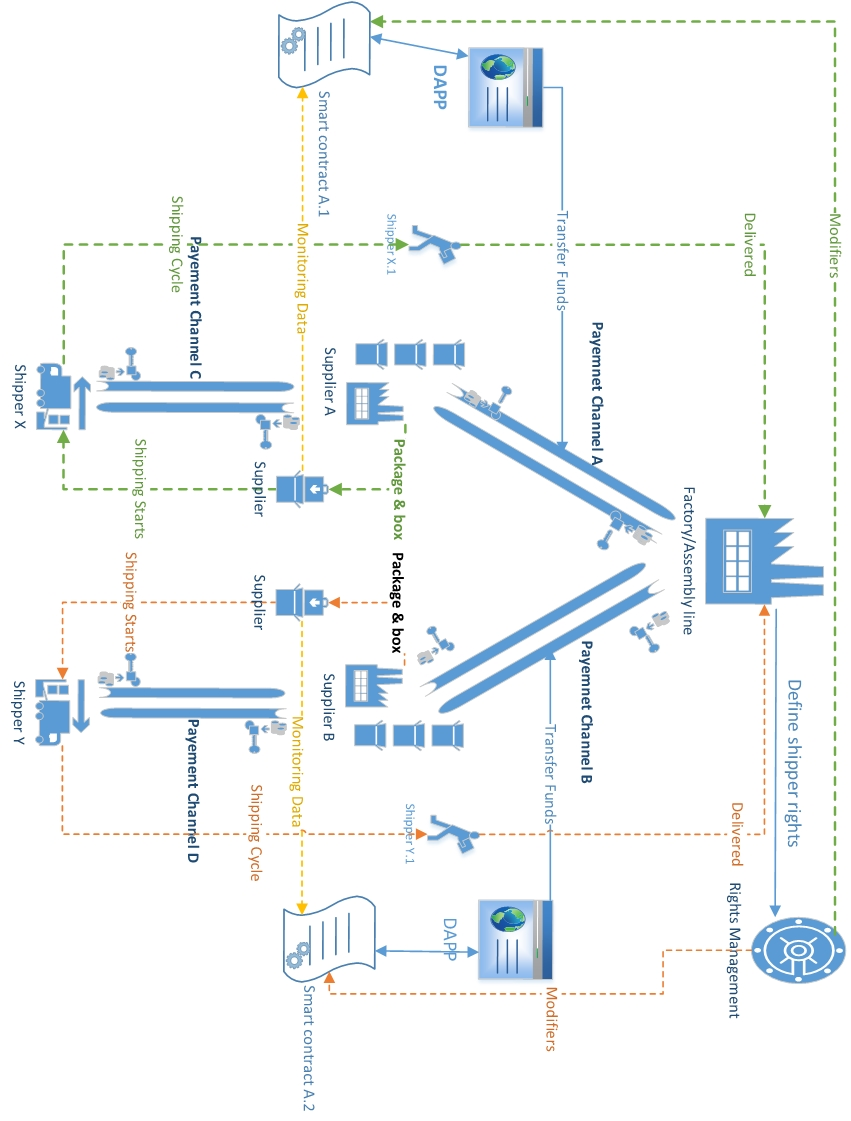
\includegraphics[width=180mm,scale=1]{figs/AbstractUC-flip}
	\caption{Shipment Tracker - Use case diagram}
	\label{fig:UseCase}
\end{figure}

\clearpage

%%%%%%Reminder: paper written use case docs is better then formal use case document I sent to the professor : rewrite and improve formal document using your paper notes

%\subsection{system Model \ requirements and assumptions} 
\subsubsection{Supply Chain LifeCycle}
In order to better explain the supply chain life cycle of our particular use case we use the simplified version of the system presented in figure \ref{fig:monitoring_subdiag}. The simplified version consists of only one supplier and shipper. The company places a new order for components with its supplier and stipulates shipping and handling constraints in the smart contract. 

\begin{figure}[h]
	\centering
    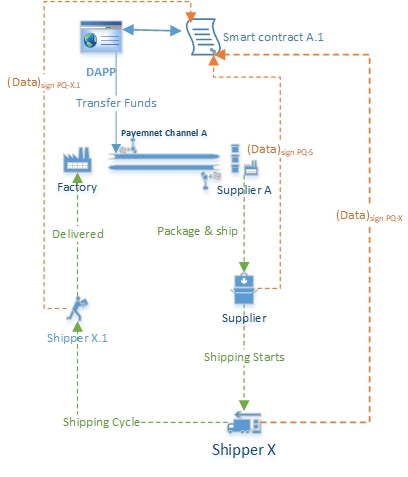
\includegraphics[width=140mm,scale=1]{figs/monitoring_subdiag}
	\caption{Supply chain Life Cycle}
	\label{fig:monitoring_subdiag} 
\end{figure}
%\clearpage

Once the order has been placed it funds the payment channel associated with its supplier. Supplier packages the components along with a tamper proof smart device which will communicate shipping data with the smart contract. The smart device is a Raspberry Pi running a custom program developed as part of this thesis to monitor package conditions and to send signed data to the smart contract. 

The data is signed with the help of a lattice based post quantum secure algorithm provided by Dr. Rachid El Bansarkhani. This algorithm protects integrity of data in the presence of post quantum adversaries. The hardware and software that collectively define a smart package will hence forth be referred to as the IoT Node. This node can be configured to send data continuously or when special events are triggered i.e. some shipping violation has occurred. We need internet connectivity throughout the shipping life cycle in order to insure monitoring data is continuously communicated with the Smart Contract and IPFS. The IoT node signs the data with the Post quantum key of the current shipper/ handler.  Monitoring starts as soon as the components are packaged in the supplier warehouse, at this time the data sent to the SC-A.1 is signed with key of the supplier. When the shipper X takes possession of the package from the supplier they scan the package. This scanning event represents changing of ownership of responsibility in the supply chain cycle which means from this point on all data sent to the smart contract will be signed with the key of the shipper X. If there is more than one shipper as show in figure \ref{fig:UseCase}, Each one scans the package to take over shipping responsibilities. In our system Smart Contracts and Dapps are responsible for catching violations and taking appropriate actions to penalize violators and compensate aggrieved parties. This brings full transparency for all stake holders in the supply chain life cycle and resolved disputes if any in an efficient and trust less manner.

\vspace{0.5cm}
\subsection{System Architecture}
The proposed system for the use case described in \ref{ST-Dapp-UC} has four main components:
\begin{enumerate}
  \item Ethereum Smart contract
  \item Raiden Payment Channels
  \item Decentralized Application or Master nodes
  \item Smart packages or IoT nodes
\end{enumerate} 

The abstract system and processes are modeled in figure \ref{fig:Abstractdesign}. Supplier and company agree on shipment conditions in the form of a business contract. These conditions are configured at the start of each shipment cycle. They are instantiated as requirements in a smart contract on the Ethereum blockchain. They cannot be altered after being set in the Smart Contract. The terms of the contract can include any type of handling constraints like exposure to high temperature, pressure, air etc. IoT enabled packages \ref{IoT-Nodes} monitor the package contents according to the defined constraints and conditions with the help of embedded sensors. They communicate shipping and logistics data with the Smart Contract. The high level functions of IoT Node or Smart Package are modeled in the abstract design diagram shown in figure \ref{fig:Abstractdesign}.
\clearpage
The Smart Contract can detect any breaches of the agreed upon terms. If any breaches are detected the system can be used to take appropriate actions to compensate or penalize the parties involved. Payment channels are established between the organization and its suppliers to handle payments efficiently. The payment channels are deployed using Raiden. A company and its suppliers agree upon a set of conditions either implicitly or explicitly at the start of each shipping cycle. The terms of conditions are instantiated in the contract with the help of Contract number or tracking number of the package. The supplier initializes the IoT module inside smart package with the tracking number. Once initialized this module contacts the smart contract to receive set of conditions associated with the tracking number. The IoT device then starts the monitoring procedure as shown in figure \ref{fig:Abstractdesign}. In order to minimize transaction costs IoT devices only sends violations to be stored in the blockchain. Full tracking logs containing sensor data like temperature, location, humidity etc are stored using IPFS. The log address or Hash is stored in the blockchain. This enables our Dapp to always have access to full logs. It can query IPFS nodes using the stored hashes to download complete logs related to any shipping cycle. Once the package is delivered the organization can check the Dapp interface to see if any conditions were violated. If no conditions were violated it transfers full amount to the supplier or the shipper. In the event that violations were detected, smart contract communicates them with the monitoring Dapp. If any violations occurred the Dapp can determine the party responsible so that appropriate actions can be taken. These actions could range from giving the supplier or shipper a bad rating to monetary punishments such as withholding payments etc. Penalties are determined based on the severity of the violations.

\begin{figure}[h]
	\centering
    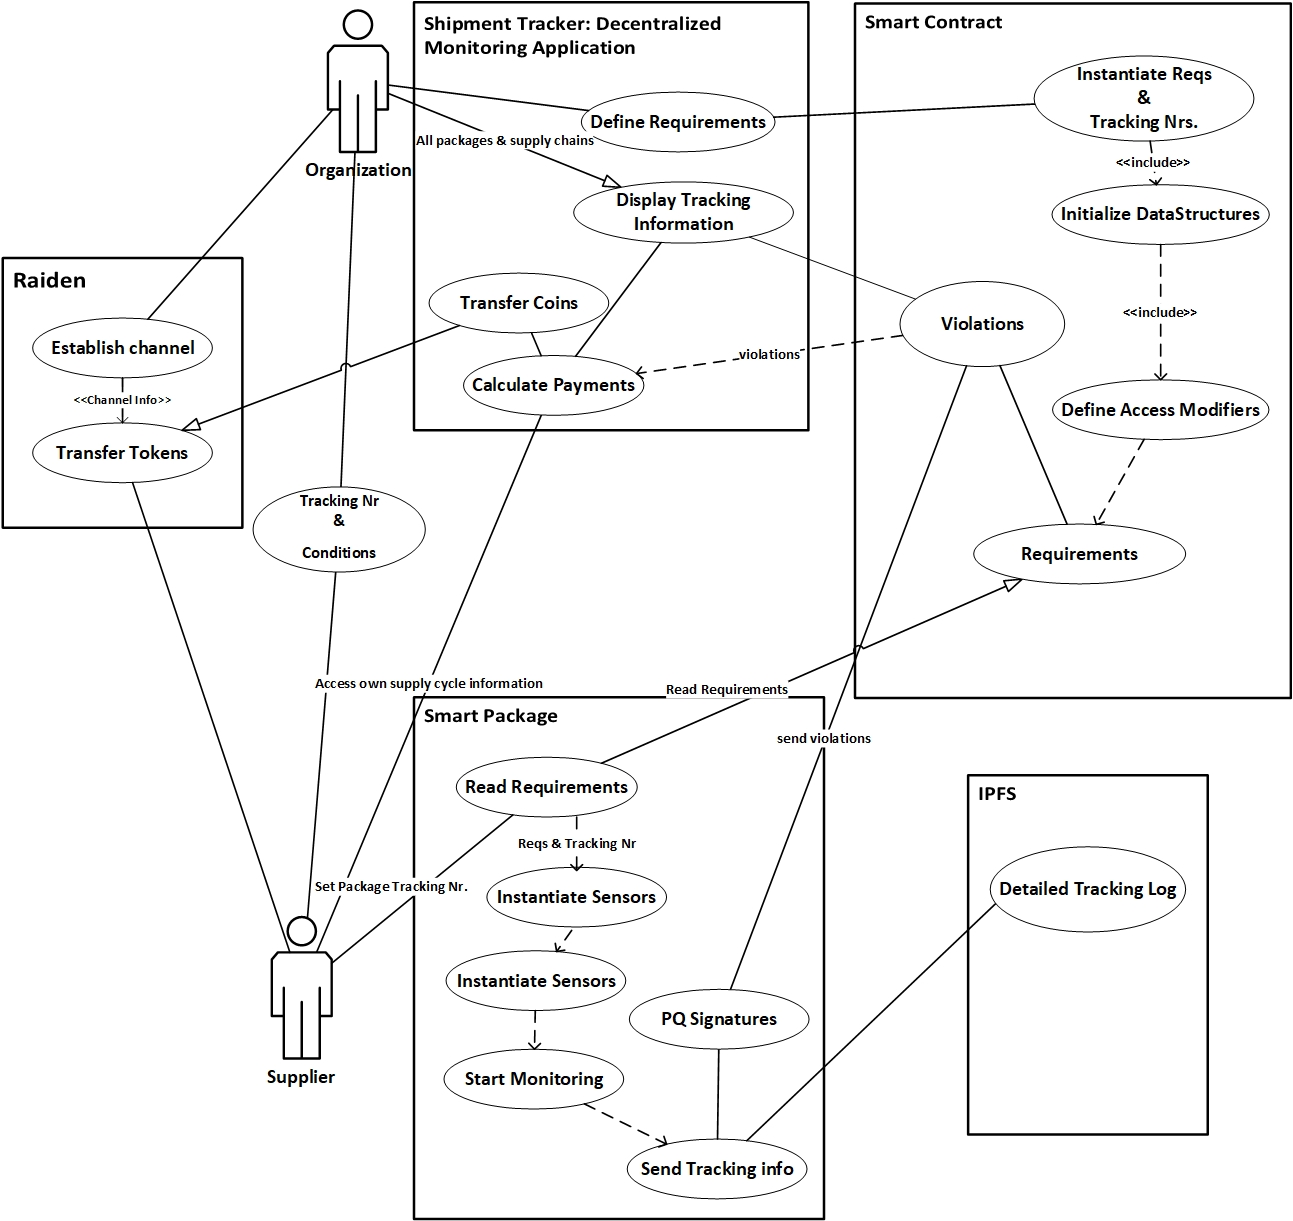
\includegraphics[width=170mm,scale=1]{figs/Abstractdesign}
	\caption{Shipment Tracker – Abstract Design}
	\label{fig:Abstractdesign}
\end{figure}
\clearpage



%\subsubsection{System Work Flow}
%Make a diagram or may be just add sequence diagram here?
%this can go into implementation chapter
%make the work flow diagram like you did for blockchain, use fileserver icon for IPFS
% Remember Registartion should be the first stage in the following figure i.e. whjere teerms are agreed, ref no / tracking nr geenrating and conditions defined 
%The IoT / tracking stage gets the condtions initializes appropriate sensors based on conditon number and starts tracking procdure.
%diagram idea mix the visio work flow stages and with flowchart like figure i.e.
%one stage shows workflow as relates to packages i.e. registering contract refnumber and defining conditions i.e. registration phase, transfering data, getting keys etc, the second stage shows smart contract / montiroing dapp monitoring data and giving out punishments and rewards etc. Last two stages are raiden and IPFS, IPFS just stores full logs, Raiden interacts with users who manually queries dapp to transfer money to shippers.
 
\subsection{Architecture - Block Diagram Overview}
Figure \ref{fig:ArchitectureBD} shows the architectural overview of our system. This system is composed of three high level components, Master Node (see \ref{MasterNode}), IoT Node (see \ref{IoTNode}), and Smart Contract (see \ref{ST-SC}).  The Master Node provides overview of the entire supply chain including activities within individual supply lines. It also handles compensation and payments to suppliers. The IoT Nodes monitor package conditions and communicates logging and tracking data with Smart Contract and IPFS. The Smart Contract provides function and logic to serve as a trustless bridge between Master Node and IoT Node. Master Node queries the smart contract to get IPFS log locations and shipping violations.
\begin{figure}[h]
	\centering
    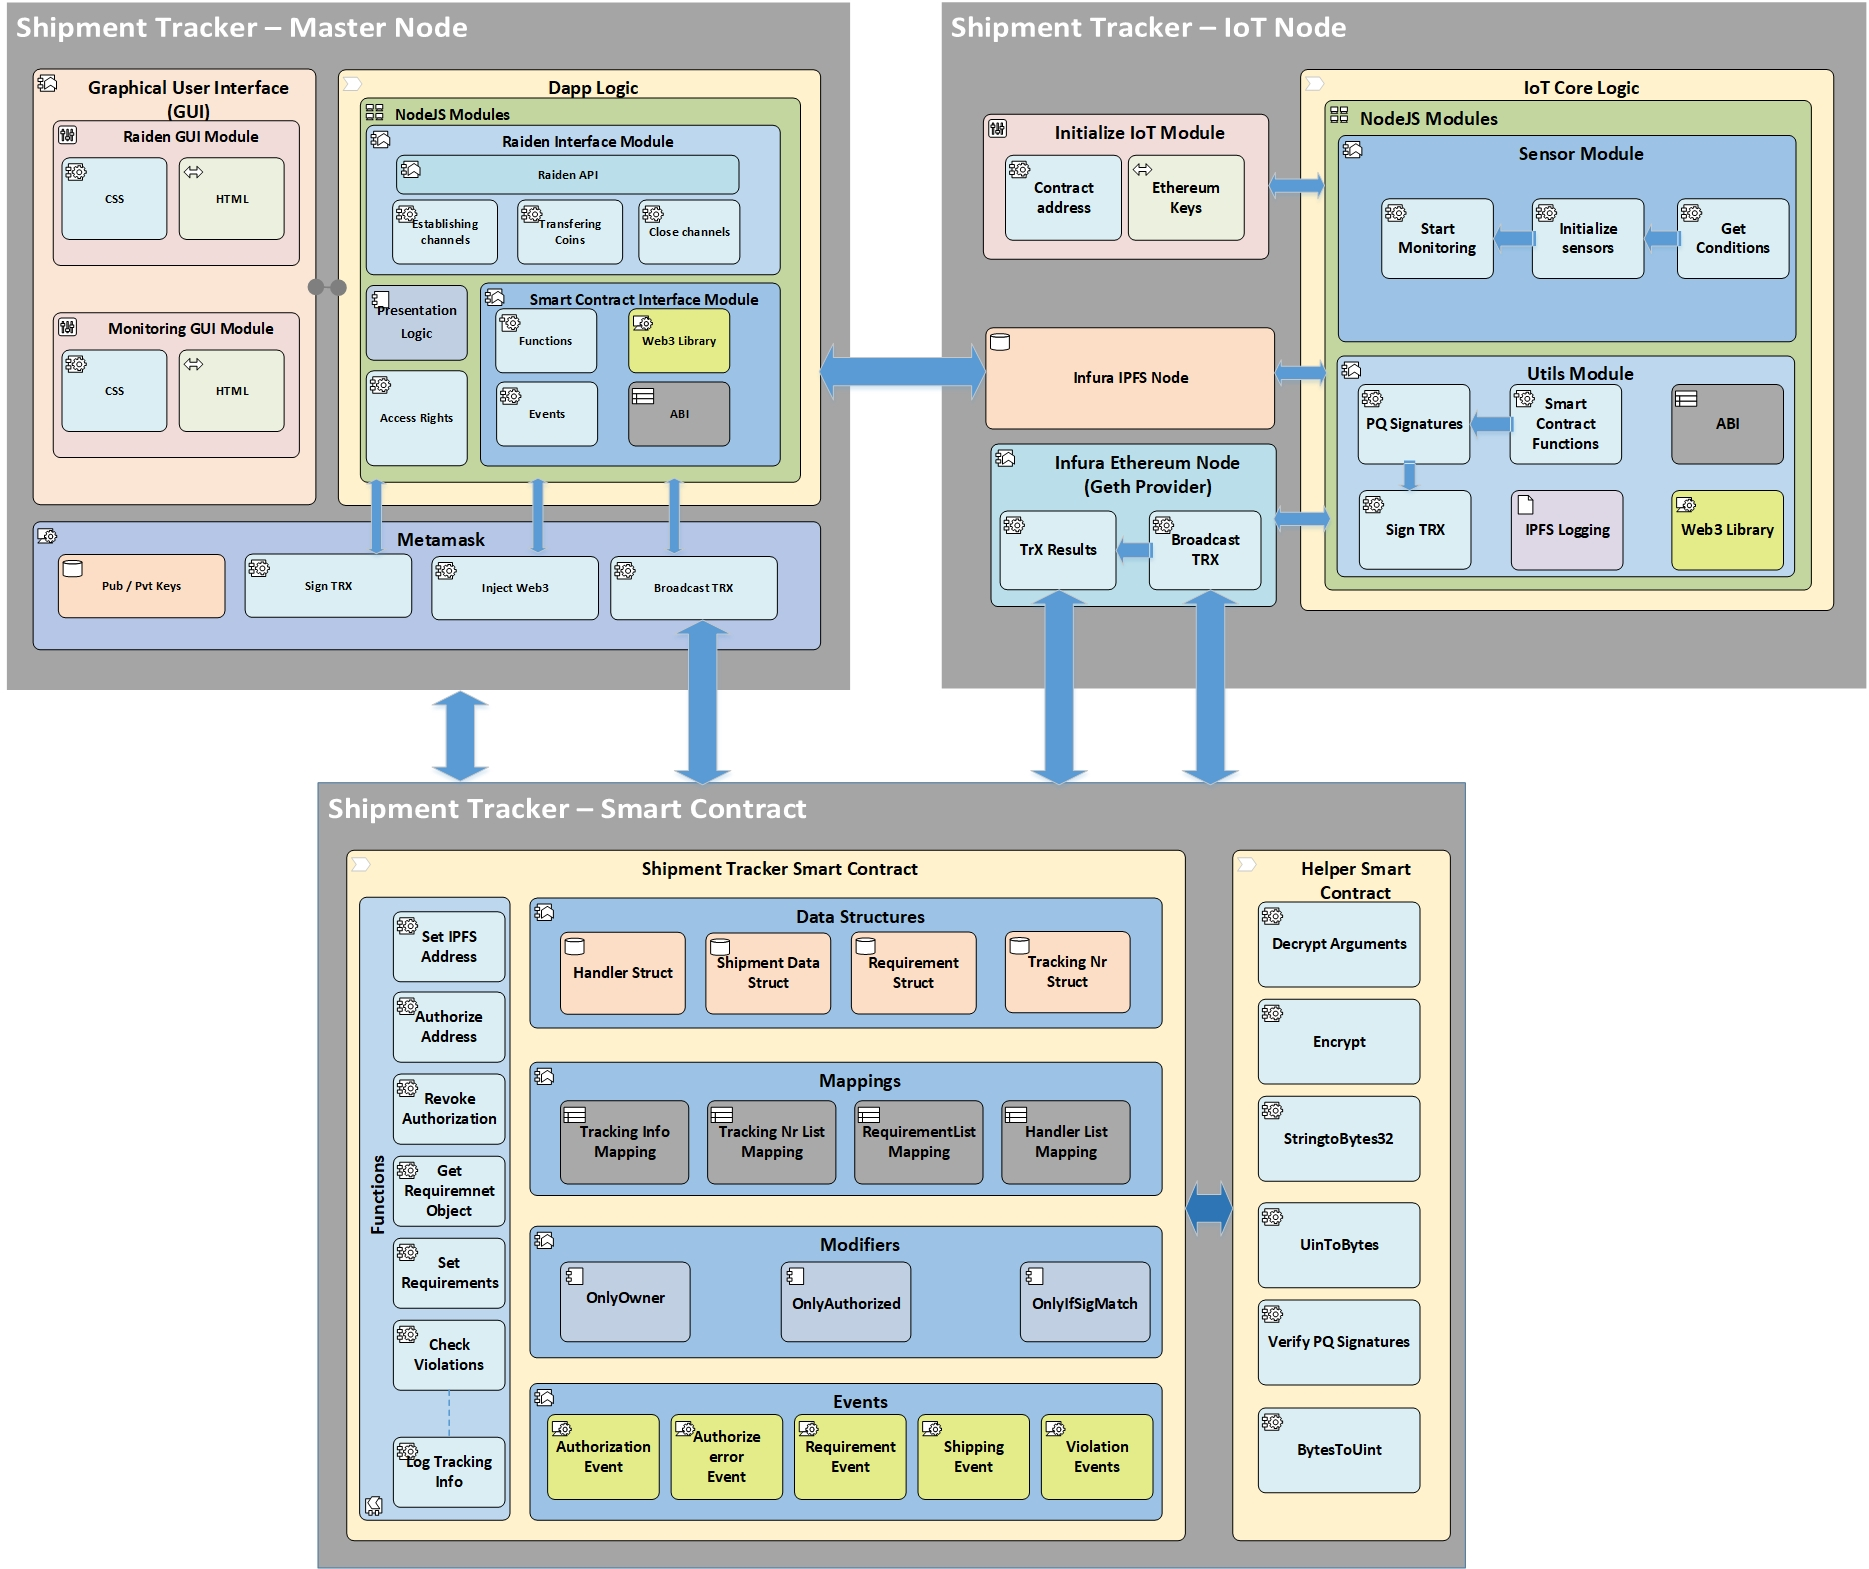
\includegraphics[width=180mm,scale=1]{figs/Blockdiagram}
	\caption{Shipment Tracker – System Block Diagram}
	\label{fig:ArchitectureBD} 
\end{figure}
\clearpage
\subsection{System Components} \label{SysComp} 
\subsubsection{Decentralized Monitoring Application - Master Node} \label{MasterNode} 
Figure \ref{fig:ArchitectureMN} details the architecture of  Master Node. This component contains the main decentralized application for monitoring all shipments across multiple supply lines. Its primary intent is to provide administrators or managers a comprehensive overview of the entire supply chain. Ethereum public key serves as the main access control mechanism in this module. It uses the public key to determine which processes or supply lines a user can view or access. The access rights are defined and stored in the smart contract. Master Node has two main sub modules. One module deals with payments and payments channels. This module relies on Raiden (see \ref{raiden}) API to establish payment channels. Raiden client must be running and fully synced with Ethereum blockchain for this module to function. The second module interfaces with the Shipment Tracker smart contract deployed on the Ethereum blockchain. The associated GUI for this module (see fig \ref{fig:ArchitectureMN}) can be used to define requirements and constraints on shipments and packages that must be followed by suppliers and shippers. This module uses web3 JavaScript library, and MetaMask browser extension to broadcast transactions to the Ethereum Blockchain. MetaMask allows us to run our Dapp Master Node without running a full Ethereum Node. The implementation details and functions of each submodule in Master Node are described in \ref{IMN}. 

\begin{figure}[h]
	\centering
    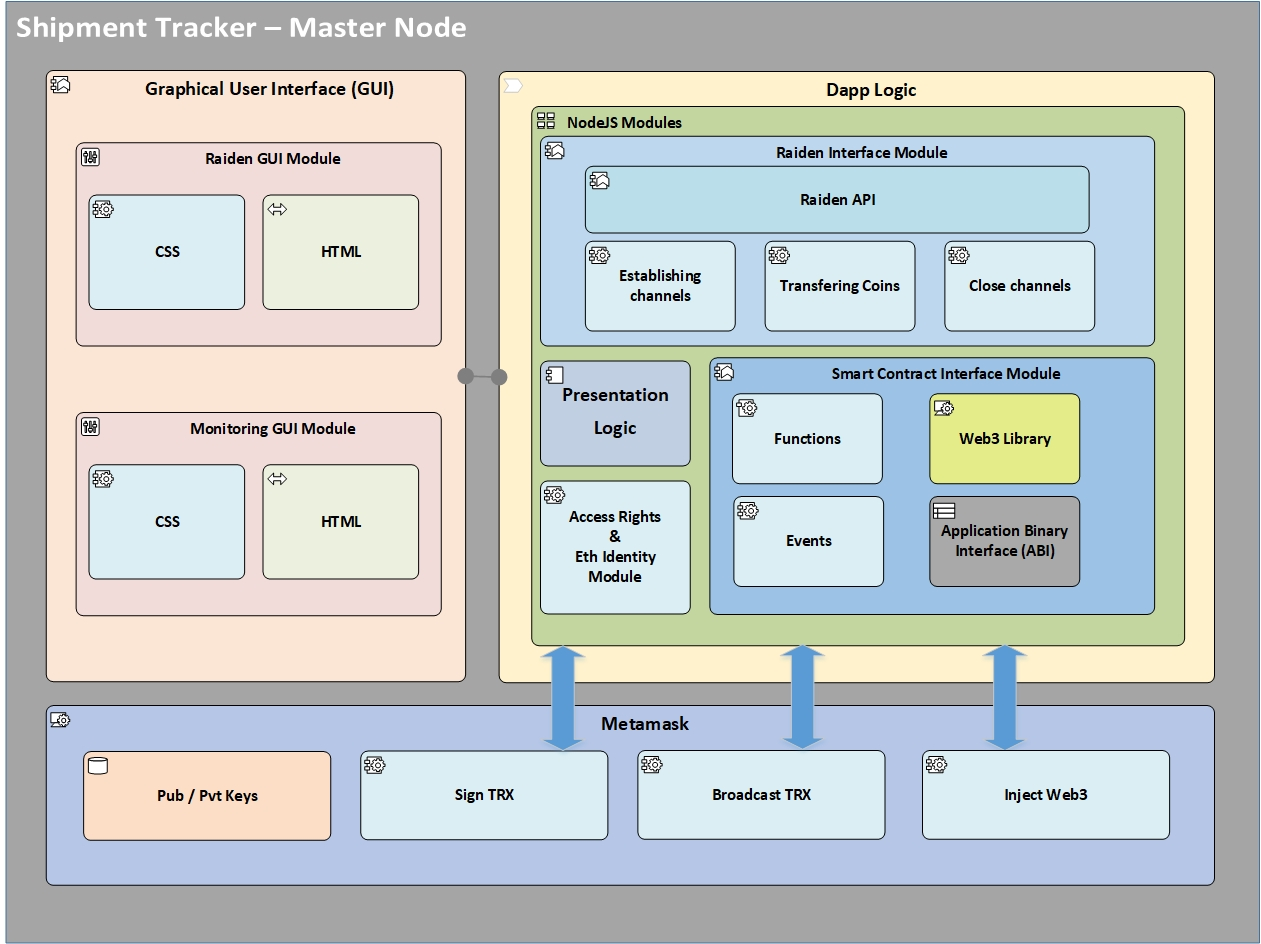
\includegraphics[width=160mm,scale=1]{figs/MasterNode-BD}
	\caption{Master Node – Block Diagram}
	\label{fig:ArchitectureMN} 
\end{figure}
\clearpage
\subsubsection{IoT Powered Smart Packages - IoT Nodes} \label{IoTNode} 
Figure \ref{fig:ArchitectureIoT} shows the architecture of IoT Nodes.  IoT Node is an embedded device with various sensors attached to monitor shipment/package conditions. IoT core logic is sub divided into three main modules Initialization Module, Sensor Module, and Utils Module. Initialization module is responsible for bootstrapping the device at the start of each new shipping cycle. It sets the shipment tracking number, sets the contract address, sets monitoring and logging intervals, and initializes the attached sensors. The device enters monitoring phase after initialization is complete. In this phase the IoT node first contacts the Shipment Tracker Smart Contract to get a list of conditions associated with the current tracking number. It then starts monitoring functions to periodically check that no condition gets violated. If any violations are found it sends them to the Smart Contract to be permanently recorded on the blockchain. In order to communicate with the blockchain we must have access to an Ethereum client. IoT nodes use the remote Ethereum Geth client provided by Infura. The client provided by Infura is just that, unlike MetaMask it does not store keys or handle transaction signing. It expects that any state altering transactions are already signed. IoT Node uses the Utils module to send signed transactions to the Geth client hosted on Infura. The Utils module is also responsible for storing shipping logs on the IPFS Network.  The implementation details of the IoT Node are explained in \ref{IoT-Nodes}.

\begin{figure}[h]
	\centering
    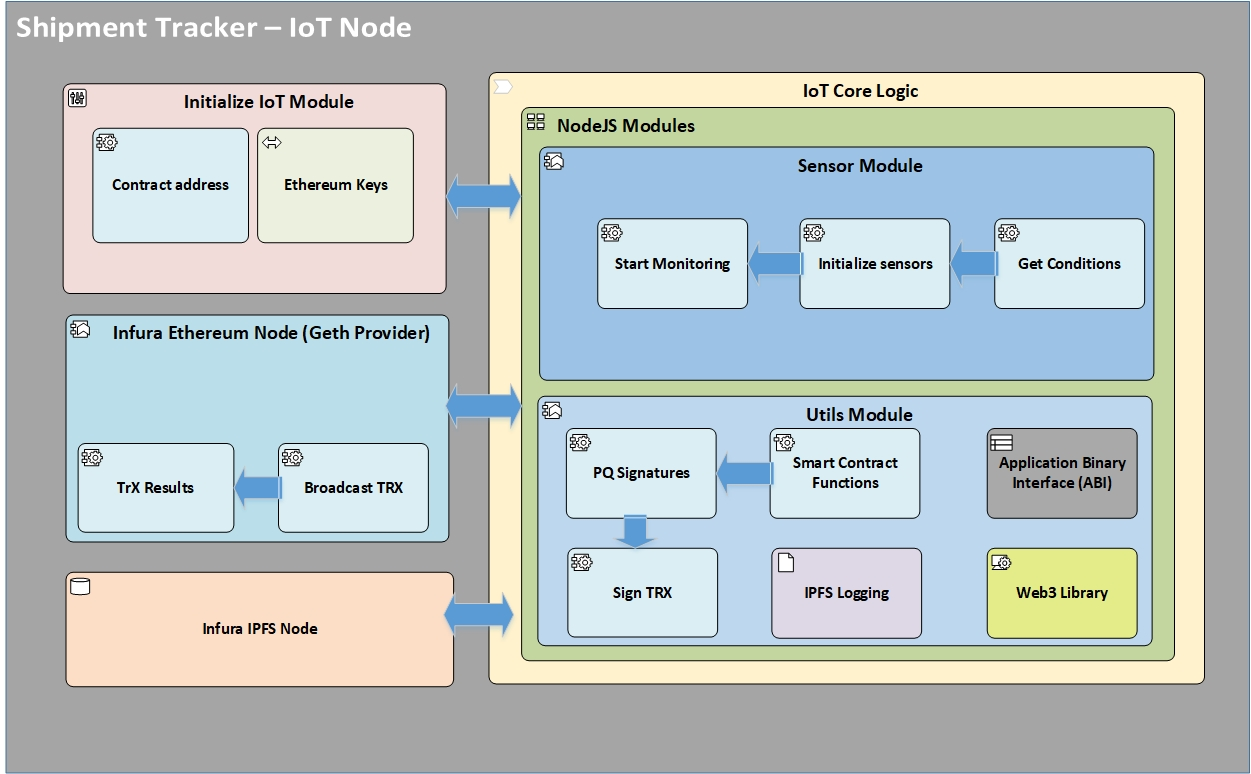
\includegraphics[width=180mm,scale=1]{figs/IoTNode-BD}
	\caption{IoT Node – Block Diagram}
	\label{fig:ArchitectureIoT} 
\end{figure}
\clearpage

\subsubsection{Shipment Tracker - Smart Contract} \label{ST-SC} 
The shipment Tracker contract is composed of several components as shown in figure \ref{fig:ArchitectureSC}. Functional logic of this contract is broken into several public, private and internal functions. Details of some of the important functional component is given in \ref{ST-SmartContract}.  The contract defines several data structures to store logical data. Shipment Data and violations sent by the IoT node are stored in ShipmentData (see \ref{ST-SmartContract}) structure, Requirements for individual shipping cycles are held in Requirements (see \ref{ST-SmartContract}) structure, and the list of authorized handlers for a individual shipments are saved in Handler (see \ref{ST-SmartContract}) structure. Modifiers in solidity modify function behavior based on some condition. In our contract modifiers are used for restricting access to certain functions and mappings to only authorized personal or devices. I use the modifier OnlyIfSigMatch to insure that data sent by IoT devices is correctly signed by the Post Quantum key of current shipper. Only verified violations are added to the blockchain. Events are used to inform the Master Node, if any state altering function was executed by the Smart Contract. The final component in figure \ref{fig:ArchitectureSC} is the library contract helper.sol. In solidity library contracts are singletons which do not store anything and can be called by any contract to extend their functionality. I developed library contract to handle post quantum signature verification. The main contract calls this library contract to verify PQ signatures. The library driven development helps to make our Smart Contract modular. It also insures that the main contract does not exceed the block limit. The current block limit on Ethereum main net is eighth million gwei.  
\begin{figure}[h]
	\centering
    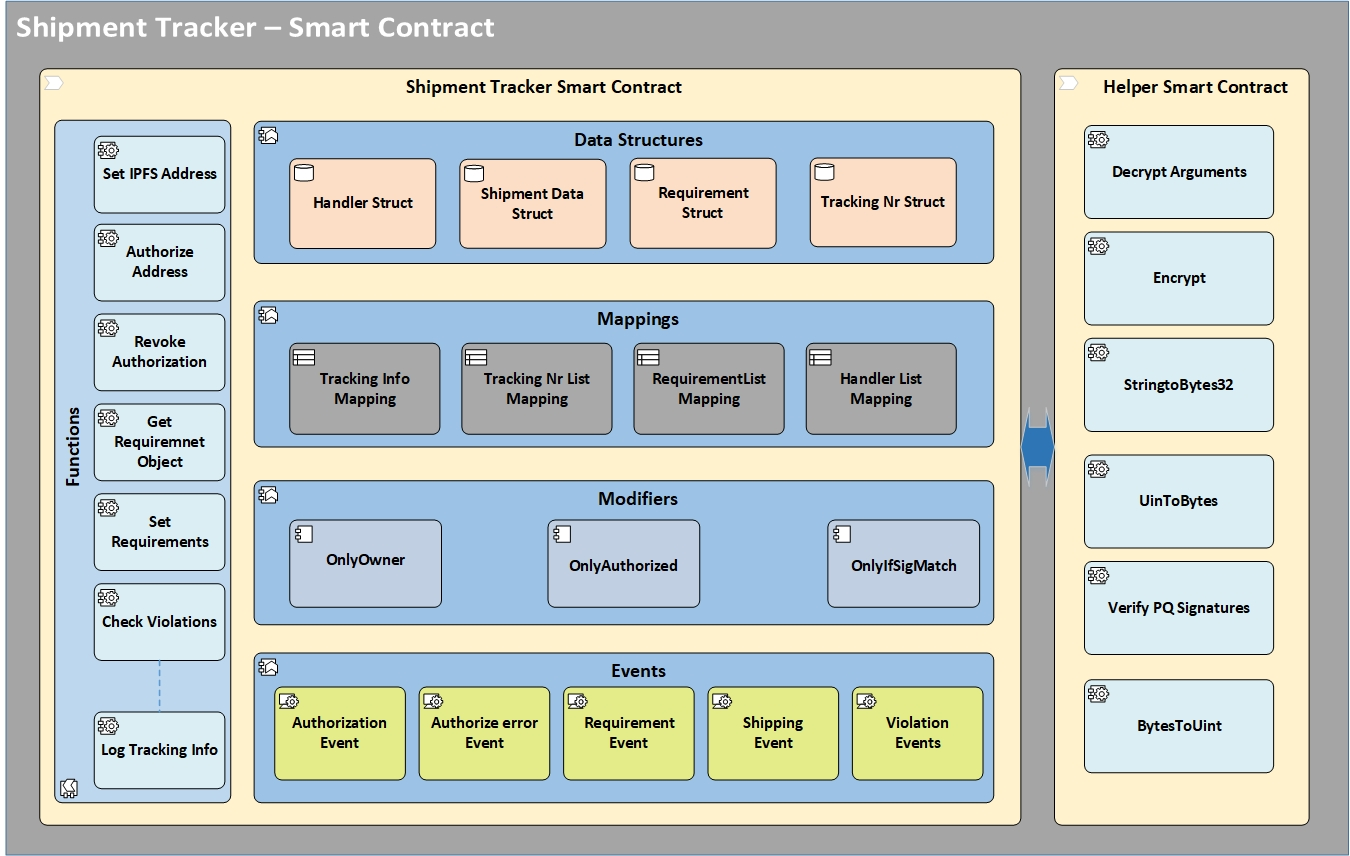
\includegraphics[width=180mm,scale=1]{figs/SC-BD}
	\caption{Smart Contract – Block Diagram}
	\label{fig:ArchitectureSC} 
\end{figure}
\clearpage



%\subsubsection{Post Quantum Module}

%say that a shipper key will be transferred when a new shipper scans the package

%\subsection{Initial Architecture}

%mention that initially each delivery cycle was going to be a single contract deployed, however this would generate lots of segregated contracts to keep track of. plus it will be very expensive in terms of operations, deployement and mantanence on public blockchain like ethereum where user pays for gas. refer to gas consumtion testing section. May even require full time blockchain developers to be able to make changes and improvements to exisiting contract templates.
%Advantage would be easiser to deal with custom situations and supply chain processes
%costs of operations would scale with ethereum prices. would make budget planning extremly difficult for organizations

%using such a systemn would create large number segregated databases which would %quickly become unmanagable for large organizations in the events of audits and analytics puposes. This will need created new buisness and IT systems for gathering managing organizing and managing distributed supply chain information.  We want distribution and redundancy of actual data and logic without adding operational overhead in terms of DB consolidtion and management on organizational level processes. The blockchain is providing an adequate solution for taking care of distribution and redundancy, Hence it was decided that it would be more worth while to invest efforts in developing a system which could serve as one generic smart contract for most of organizational needs. refer to section below.  
\section{Implementation Details}
give the algorithm that professor told you
\subsection{Hardware Setup}
Master Node
PI Node
\subsection{Software Architecture}
\subsubsection{Master Node}
give class diagrams and some details about monitoring dapp

\subsubsection{Sensor Nodes}
give class diagrams and some details about sensor nodes
\subsubsection{Integrated Payment Solution}

\subsection{Securing the System Against Post Quantum Adversaries}
\section{Testing and Results}
\subsection{Testing Environment}
ropsten, pi, ganachi,IPFS
\subsection{Results}
\subsubsection{Unit Testing}
\subsubsection{Scenario - I}
\subsubsection{Scenario - II}
\subsubsection{Scenario - III}
\subsection{Evaluation}
\subsubsection{Gas Consumption}
deployement,each tx cost, word about gas price etc
\subsubsection{Transaction Verification Time}
dependent on gas price, network congestion etc
\section{Conclusion and Future Work}
\ points to elabortae
Make the design flexible i.e. so that it does not require always on internet connection.
i.e. it communicates shipping and logistical data whenever internet or network connection is available.
Use Perun to get the entire smart contract offchain to reduce dependency on on chain and resiliance against network congestions.
etct etch
\\ log files uploaded to IPFS can be encrypted with either public key or secret key techniques to provide complete data security 
further try and solve the confidentiality issue.?
To conclude\ldots
Conclusion

In this thesis we developed a proof of concept system , This demonstrated the usefulness of such a system. A corporate or enterprise level solution will need additional supporting technologies and systems for it function smoothly. One area of improvement would be integrating RF chips in the IoT nodes that shippers Scan using their phones or RF readers to send change in shipper notifications etc. We could develop a smart phone application which could be used to scan packages and get all relevant information using NFC or Bluetooh. Managers and Supply chain engineers can use this application to subscribe to important events such as change in shipper or custom checks etc. to get real time information every where. This could help them plan better supply chain processes in the future.


Our system can reduce cost, increase efficency, and increase transparency. It reduces cost by increasing automation, data is sent autmatically from IoT nodes to the blocckhain,   The company and shippers does not need to hire dedicated persons for entering data in suplly chain monitoring systems which is the case in traditional systems. Shippers and Company reps can subscribe to important events.

Efficency is increased, by eliminated human errors, and providing real time critical data to the relevant stake holders. 

This system establishes trust between parties by giving every stake holder access to the same information. Shippers, suppliers and company execs all have access to the same data, and the system is not under the control of any one party.



\subsection{Benefits}
%Benefits
I.e allows complete transparency to all participants of the supply chain. Enables / Gives end users or customers to have complete confidence that the product was stored, shipped and handled in accordance to strict safety standards and regulations. The transparency brought by this solution to  the supply chain life cycle makes the job of government regulators and safety inspectors much simpler.

Although our test case calls for only monitoring environmental conditions and location of a shipment or package, This technology can be easily extended to monitor other critical events like custom checks or quality checks etc. This has the potential to reduce delays at borders, custom procedures could be automated with IoT node securely communicating custom declarations to the systems at the border. Similarly quality and compliance checks can be expedited, IoT package would send quality and comliance information to the concerned parties in advance or on demand. We can greatly reduce the number of humans involved in these processes by automating
processes like custom declarations and compliance certifications.
   
Improvements 
before shipping starts the raspberry pi must be configured with the correct tracking number. The supplier must do this manually, how ever this can be automates easily by giving a static device number to each sensor node and then assigning new tracking number to a device each time raspbery pi / iot node starts. Wehn an IoT node starts it will query the remote server with its deviceID to get a tracking number for the new shipping cycle. 

We can integrate a supplier rating system in our dapp to keep track of ratings. The supplier and shipper would be given a bad rating for less svere violations. Each violation carries a severity level i.e. medium to low would result in a bad rating. Organization can use the ratings to keep track of the quality of service provided by the shipper or supplier. 
Mention another benefit of using a private blockchain would be to 

%%%%%%%%%%%%%%%%%%%%%%%%%%%%%%%%%%%%%%%%%%%%%%%%%%%%%%%%%
%%%%%%%%%%%%%%%%%%%%%%%%%%%%%%%%%%%%%%%%%%%%%%%%%%%%%%%%%
  
\appendix  
% Adjust page numbering (optional)
\pagenumbering{Roman}
 
\newpage
\phantomsection
\listoffigures 
\newpage
\phantomsection
\listoftables
\newpage

% Create bibliography
\phantomsection
\bibliographystyle{alpha}
% bibliography file title
\bibliography{literatur}


%%%%%%%%%%%%%%%%%%%%%%%%%%%%%%%%%%%%%%%%%%%%%%%%%%%%%%%%%
%%%%%%%%%% Appendix %%%%%%%%%%%%%%%%%%%%%%%%%%%%%%%%%%%%%
%%%%%%%%%%%%%%%%%%%%%%%%%%%%%%%%%%%%%%%%%%%%%%%%%%%%%%%%%
\newpage
\section{Appendix Stuff}

the Appendix
\section{Acronyms}
\begin{acronym}
 \acro{DDOS}{Distributed Denial of Service} 
 \acro{Dapps}{Decentralized Applications} 
 \acro{Altcoins}{All other coins besides Bitcoin}
 \acro{JIT}{Just In Time}
 \acro{IoT}{Internet of Things}
 \acro{SCM}{Supply Chain Management}
 \acro{DLT}{Distributed Ledger Technology}
 \acro{TX}{Transaction}
 \acro{TX}{Transaction}
 \acro{POW}{Proof of Work}
 \acro{POS}{Proof of Stake}
 \acro{TPS}{Transactions per second}
 \acro{MTX}{Microtransactions}
 \acro{BTC}{Bitcoin}
 \acro{PoR}{Proof of Replication}
 \acro{PoS}{Proof of Storage}
\end{acronym}
%%%%%%%%%%%%%%%%%%%%%%%%%%%%%%%%%%%%%%%%%%%%%%%%%%%%%%%%%
%%%%%%%%%%%%%%%%%%%%%%%%%%%%%%%%%%%%%%%%%%%%%%%%%%%%%%%%%

\end{document}
